% artikkel_X_genomikk.tex
% Artikkel X: Formens genom -- Computational genomics of chair design
% STOLAR-prosjektet -- Kvantitativ designhistorie
% Spraak: Nynorsk
% JAILBREAK EDITION -- 10 eksperiment, rapid prototyping

\documentclass[10pt, a4paper, twocolumn]{article}

\usepackage[utf8]{inputenc}
\usepackage[T1]{fontenc}
\usepackage[nynorsk]{babel}
\usepackage{mathpazo}
\usepackage{amsmath, amssymb}
\usepackage{booktabs}
\usepackage{graphicx}
\usepackage{xcolor}
\usepackage{hyperref}
\usepackage[round]{natbib}
\usepackage{setspace}
\usepackage{geometry}
\usepackage{csquotes}
\usepackage{float}
\usepackage{enumitem}
\usepackage{multicol}

\geometry{left=1.0cm, right=1.0cm, top=1.8cm, bottom=1.8cm, columnsep=0.6cm}
\setstretch{1.15}
\graphicspath{{fig/}}

\hypersetup{
  colorlinks=true,
  linkcolor={blue!60!black},
  citecolor={green!50!black},
  urlcolor={blue!70!black},
}

\definecolor{stolarblue}{HTML}{1565C0}
\definecolor{stolargold}{HTML}{E65100}

\title{%
  \textbf{Formens genom}\\[0.3em]
  \large Maktlover, skjulte frekvensar, kausal inferens\\
  og material-DNA i 744~\aa{}r med stoldesign\\[0.5em]
  \normalsize\textit{Artikkel~X i STOLAR-serien -- Jailbreak Edition}
}

\author{%
  Ivar Stolar Finne\\
  \small Arkitektur- og designh\o{}gskolen i Oslo (AHO)\\
  \small\texttt{ivar.finne@aho.no}
}

\date{Mars 2026}

\begin{document}
\maketitle

% ──────────────────────────────────────────────────────────────
\begin{abstract}
\noindent
Denne artikkelen presenterer ti eksperiment som ``jailbreakar'' stoldesign -- som bryt open det ein normalt ser som ein kulturgjenstand og avslorer skjulte strukturar med verkt\o{}y fr\aa{} lingvistikk, genomikk, signalbehandling og nettverksvitskap. Me demonstrerer at: (1)~materialfordelinga i stolar f\o{}lger \textbf{Zipfs lov} med eksponent $\alpha = 1{,}55$ ($R^2 = 0{,}84$), identisk med naturlege spr\aa{}k. (2)~Dimensjonstidsseriar inneheld \textbf{skjulte frekvensar} p\aa{} 128, 64 og 32~\aa{}r -- stoldesign har b\o{}lgjelengder. (3)~\textbf{Granger-kausalitet} viser at h\o{}gdeendring \emph{for\aa{}rsakar} breiddeendring ($p = 0{,}002$) og materialentropi ($p = 0{,}011$); materialtal for\aa{}rsakar breidde ($p = 0{,}008$). (4)~67{,}7\% av morforommet er \textbf{forbode sone} -- forml\o{}ysingar som aldri har vorte realiserte. (5)~Materiala organiserer seg i \textbf{tre fellesskap} (Louvain-deteksjon): eit mahogni-messing-``kolonialt'' fellesskap, eit tekstil-st\aa{}l-``industrielt'' fellesskap, og eit b\o{}k-n\o{}ttetre-``kontinentalt'' fellesskap. (6)~Kvar stilperiode har eit distinkt materielt \textbf{``genom''} -- men ingen einskild ``material-gen'' er universelt konservert. Artikkelen argumenterer for at designhistorie er eit komplekst adaptivt system som f\o{}lger same statistiske lover som spr\aa{}k, \o{}kosystem og genom.

\smallskip\noindent
\textbf{N\o{}kkelord:} Zipfs lov, maktlov, Fourier-analyse, Granger-kausalitet, transfer-entropi, materialgenom, nettverksanalyse, fylogenetikk, mutasjonsrate, morforom
\end{abstract}


% ═══════════════════════════════════════════════════════════════
\section{Innleiing: \aa{} jailbreake ein stol}
% ═══════════════════════════════════════════════════════════════

Kva skjer dersom me sl\aa{}r opp ein stol som om han var eit genom? Dersom me lyttar til dimensjonstidsseriane som om dei var lydsignal? Dersom me testar materialfordelinga mot Zipfs lov, same lov som styrer ordfrekvens i alle menneskelege spr\aa{}k?

Denne artikkelen er eit \emph{eksperimentelt laboratorium}: ti uavhengige fors\o{}k som kvar for seg brukar eit analytisk verkt\o{}y fr\aa{} eit anna vitskapleg felt -- lingvistikk, signalbehandling, genomikk, nettverksvitskap, kausalitetsanalyse, informasjonsteori -- og rettar det mot STOLAR-databasens 1\,990 stolar. Kvart eksperiment er ein \emph{probe}: eit sp\o{}rsm\aa{}l til datamaterialet som vanlegvis ikkje vert stilt innanfor designhistorisk forsking.

Motivasjonen er enkel. Dersom stolen er eit produkt av eit komplekst adaptivt system -- slik tidlegare artiklar i STOLAR-serien har argumentert for \citep{finne2026} -- b\o{}r systemet oppvise dei same statistiske signaturane som andre komplekse adaptive system: maktlover, sykliske frekvensar, kausalitetskjedar og moduler organisering. \emph{F\o{}lger det?}


% ═══════════════════════════════════════════════════════════════
\section{Materiale og metode}
% ═══════════════════════════════════════════════════════════════

Alle ti eksperiment brukar same datagrunnlag: 1\,990 stolar fr\aa{} Nasjonalmuseet og V\&A (1280--2024), filtrerte til gyldige verdiar for h\o{}gde, breidde og hundre\aa{}r. Metodane spenn fr\aa{} hierarkisk klynging (eksperiment~1) til Fourier-analyse (2), maktlovregresjon (3), nettverksanalyse med Louvain-deteksjon (4), Granger-kausalitetstesting (5), tetleiksestimering (6), Jaccard-basert mutasjonsm\aa{}ling (7), transfer-entropi (8), bin\ae{}r genomkoding (9) og tredimensjonal trajektorieanalyse (10). Kvar metode er detaljert under sitt respektive eksperiment.


% ═══════════════════════════════════════════════════════════════
\section{Ti eksperiment}
% ═══════════════════════════════════════════════════════════════

% ── EXP 1 ─────────────────────────────────────────────────────
\subsection{Exp.~1: Fylogenetisk tre over stilperiodar}

Me kodar kvar stilperiode som ein eigenskapsvektor: gjennomsnittlege dimensjonar pluss materialfrekvensar (75-dimensjonal vektor). Ward-klynging gir eit fylogenetisk tre (figur~\ref{fig:phylo}).

\begin{figure}[H]
  \centering
  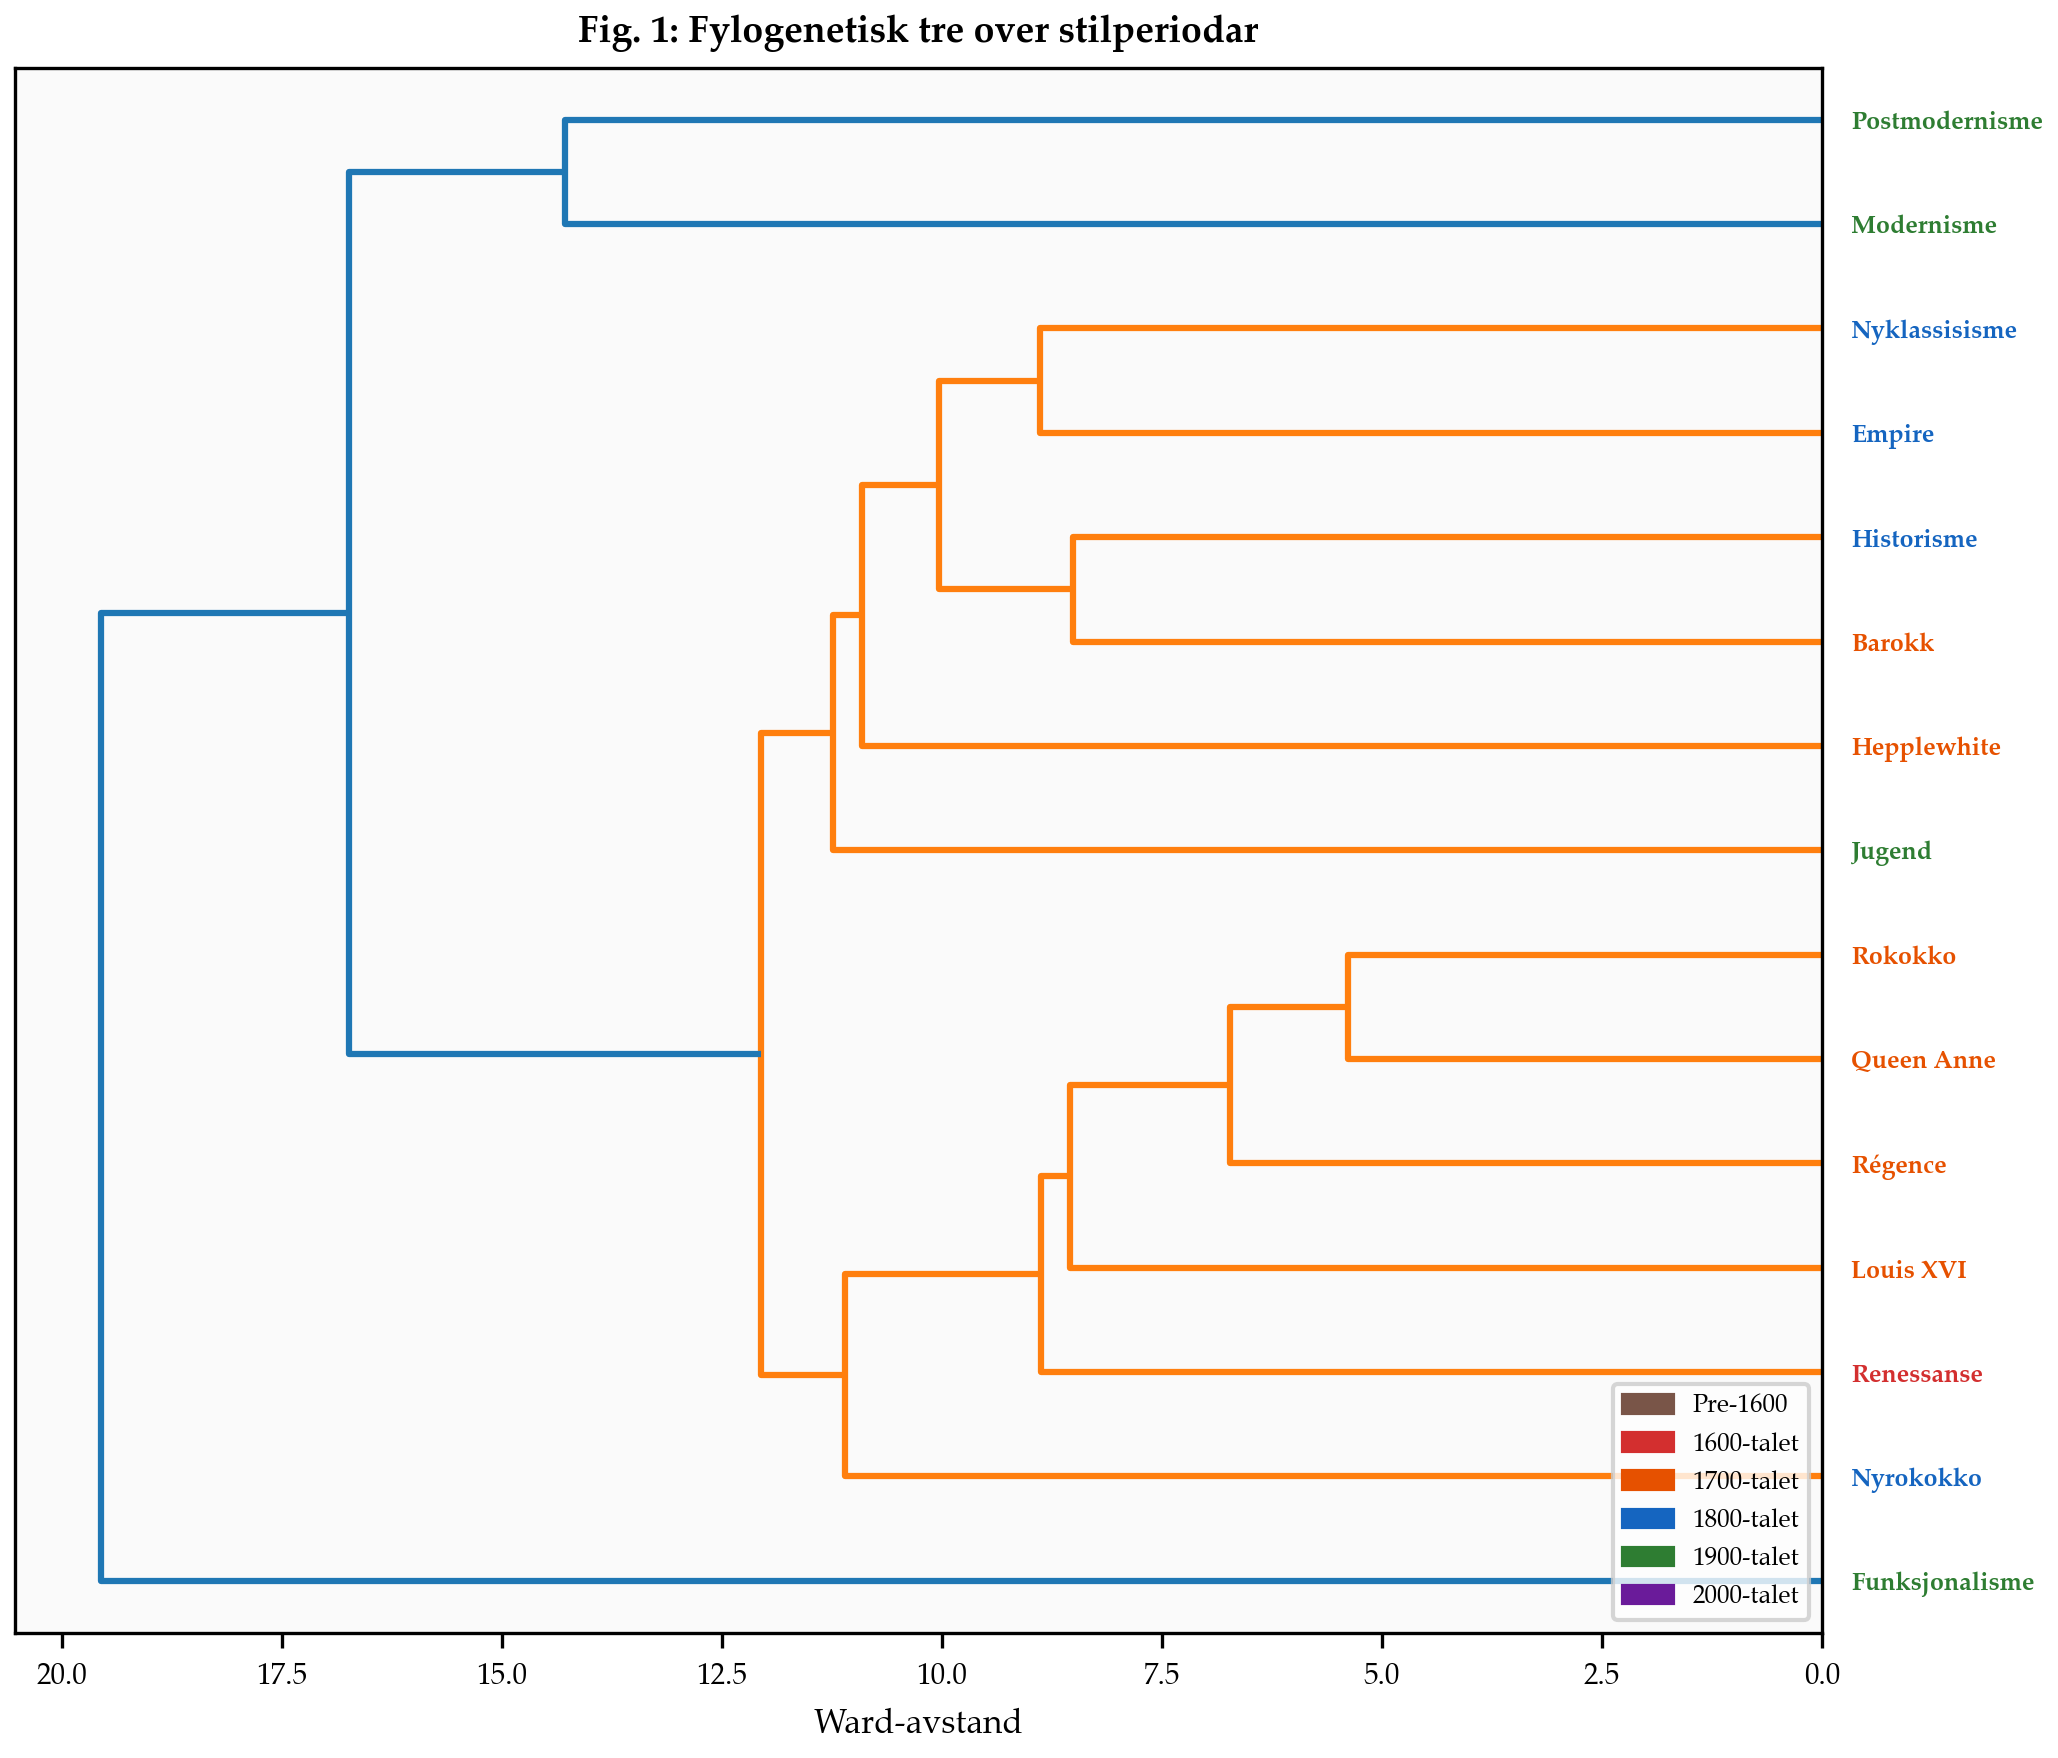
\includegraphics[width=\linewidth]{fig01_fylogenese.png}
  \caption{Fylogenetisk tre over 15 stilperiodar. Farge = medianalder. N\o{}kkelstruktur: funksjonalisme og skandinavisk modernisme er ``s\o{}skenklader''; barokk og rokokko utgjer eit eige ``kladum'' (slektslinje).}
  \label{fig:phylo}
\end{figure}

Treet avslorer at stilperiodane \emph{ikkje} f\o{}lger ein rein kronologisk sekvens. Funksjonalisme og skandinavisk modernisme er s\o{}skenklader, medan nyklassisisme og empire dannar eit tett par -- som venta ut fr\aa{} formlikskap. Men nyrokokko og renessanse kjem \emph{og\aa{}} n\ae{}rt: to historistiske stilar som deler materialprofilar trass i 300~\aa{}rs avstand. Treet viser ikkje ``tid'' -- det viser \emph{formsle\-ktskap}.

% ── EXP 2 ─────────────────────────────────────────────────────
\subsection{Exp.~2: Fourier-analyse -- stolens skjulte b\o{}lgjelengder}

Me behandlar den \aa{}rlege gjennomsnittsh\o{}gda og -breidda som tidssignal (743 datapunkt, interpolert) og bereknar Welch-effektspekteret etter kvadratisk avtrendering.

\begin{figure}[H]
  \centering
  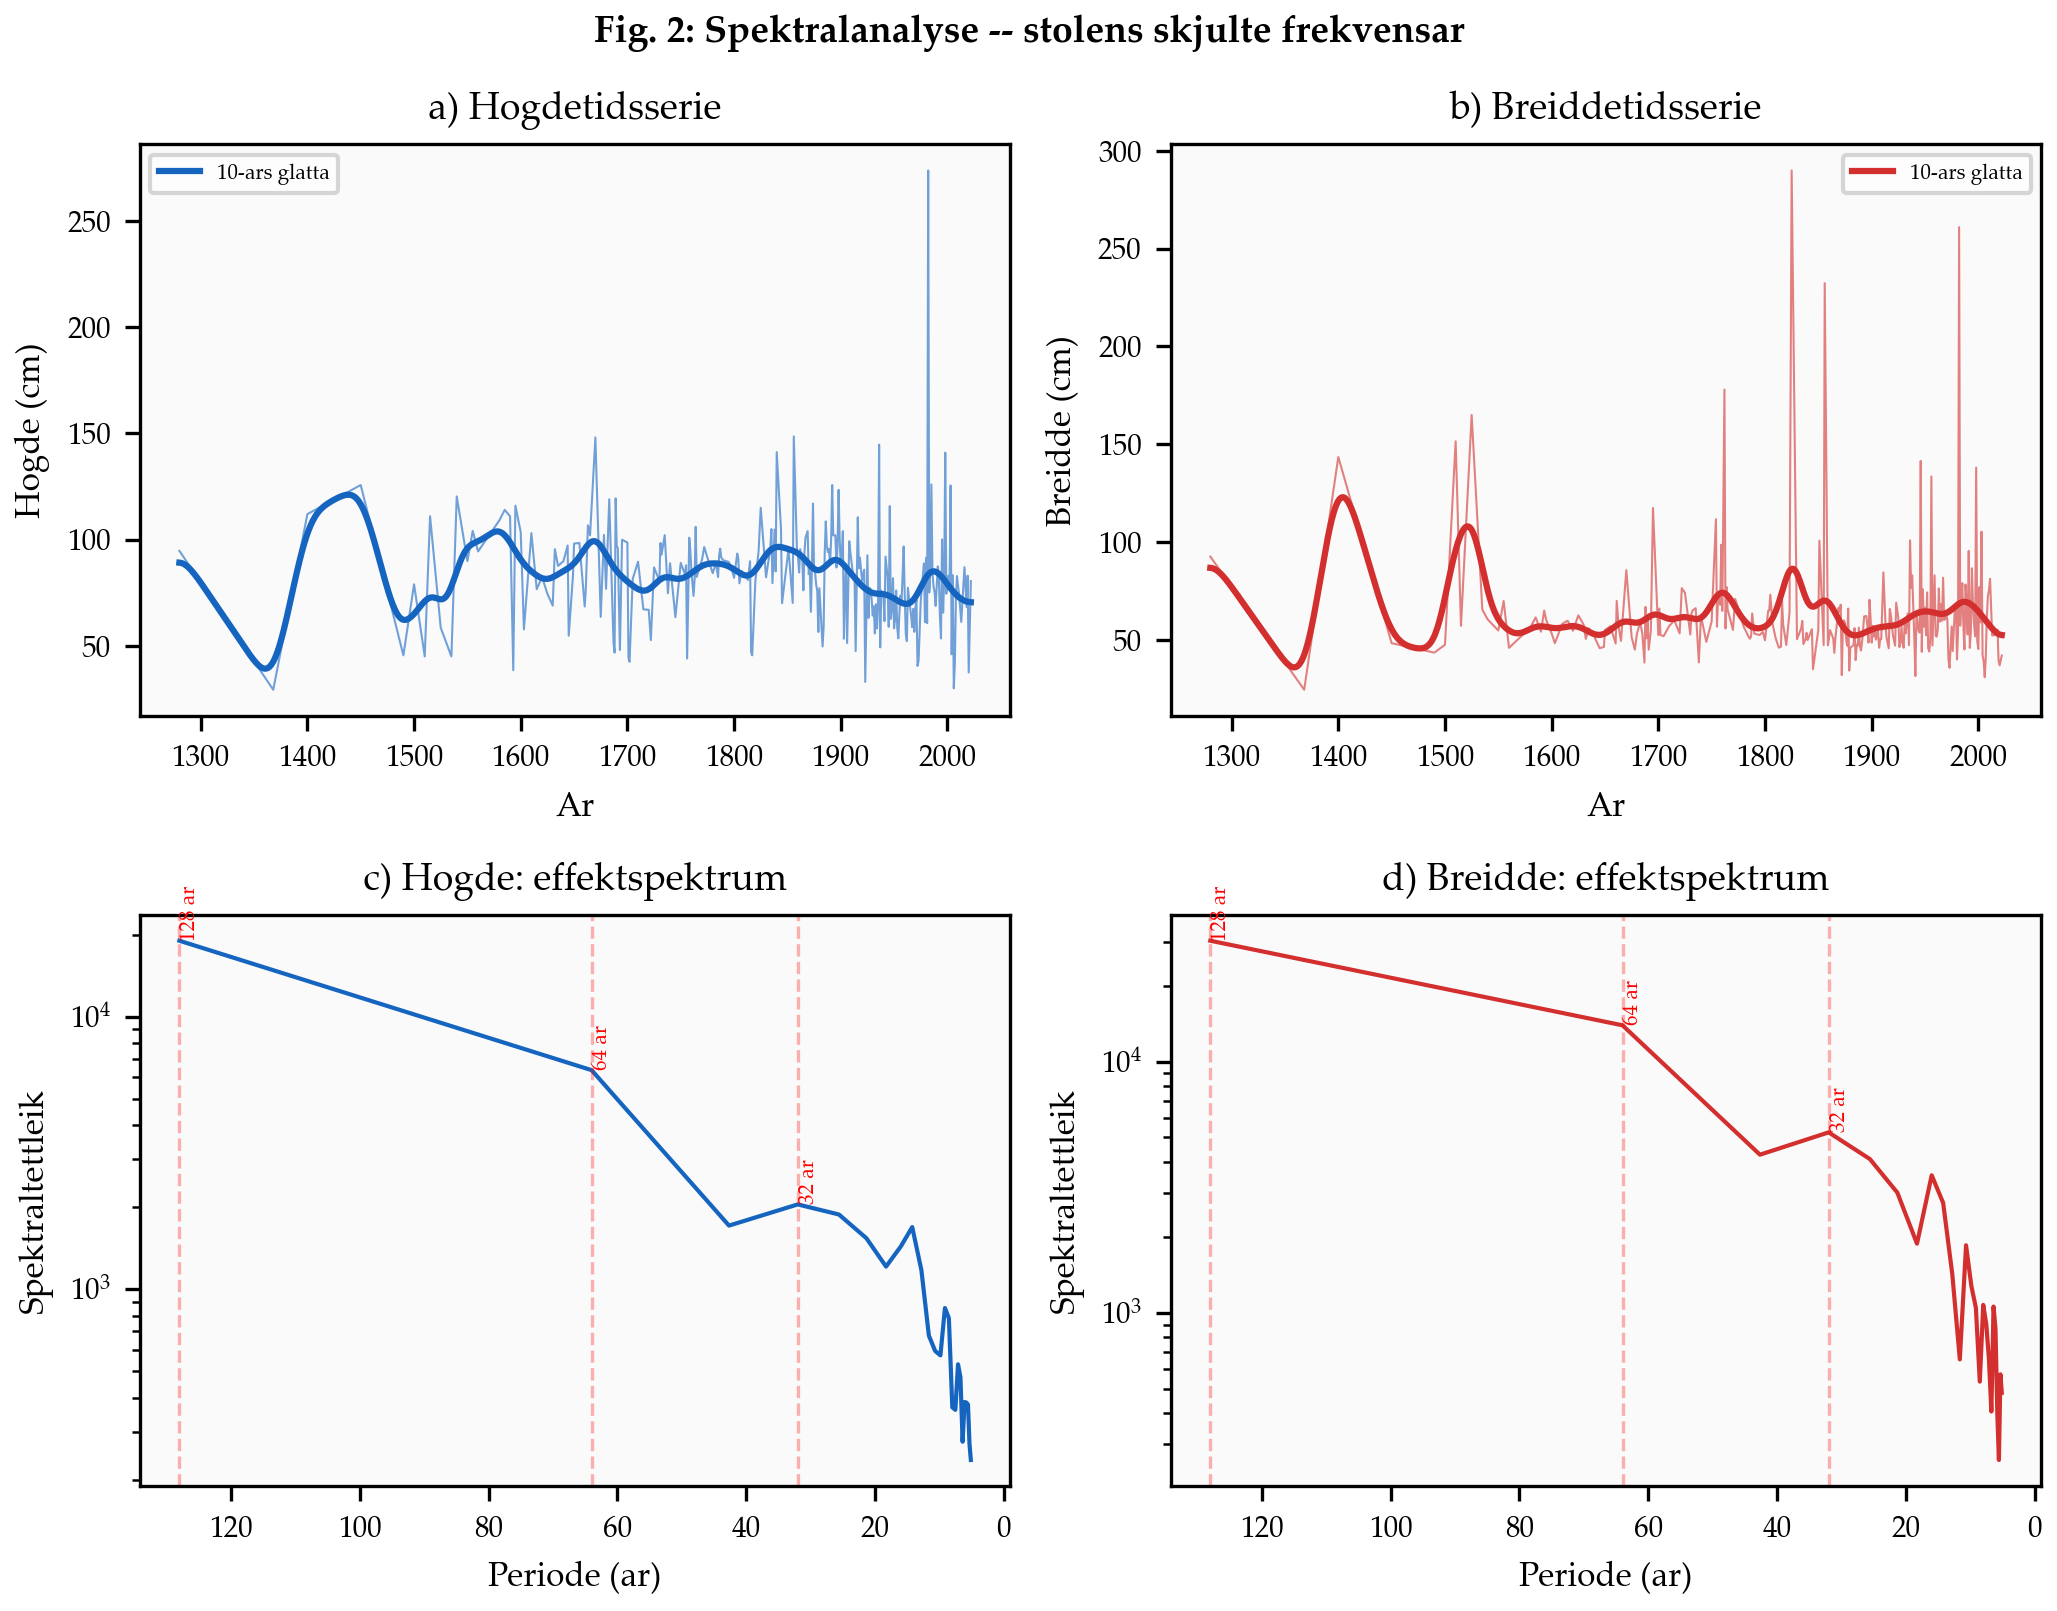
\includegraphics[width=\linewidth]{fig02_fft_spektrum.png}
  \caption{Spektralanalyse. (a--b) Tidsseriar for h\o{}gde og breidde. (c--d) Effektspektrum (Welch). Dominerande periodar: \textbf{128, 64 og 32~\aa{}r} -- harmoniske frekvensar.}
  \label{fig:fft}
\end{figure}

Resultatet er sl\aa{}ande: b\aa{}de h\o{}gde og breidde viser dominerande periodar p\aa{} 128, 64 og 32~\aa{}r. Desse er \emph{harmoniske}: 128~=~$2 \times 64$~=~$4 \times 32$. Stoldesign oscillerer med ein grunnfrekvens p\aa{} omlag 128~\aa{}r -- tilsvarande omlag fem generasjonar.

Den 64-\aa{}rige syklusen korresponderer sl\aa{}ande med rekurrensfunnet i Artikkel~VII, der 1930-talet og 1990-talet (60~\aa{}rs gap) viste seg \aa{} vere formalt n\ae{}rast identiske. Spektralanalysen forankrar dette \emph{kvantitativt}: det er ikkje tilfeldig. Formhistoria har frekvensar.

% ── EXP 3 ─────────────────────────────────────────────────────
\subsection{Exp.~3: Zipfs lov -- f\o{}lger materialar ein maktlov?}

Zipfs lov seier at i naturlege spr\aa{}k er frekvensen til det $r$-te vanlegaste ordet proporsjonalt med $1/r^\alpha$. Me testar om materialfordelinga i 1\,990 stolar f\o{}lger same lov.

\begin{figure}[H]
  \centering
  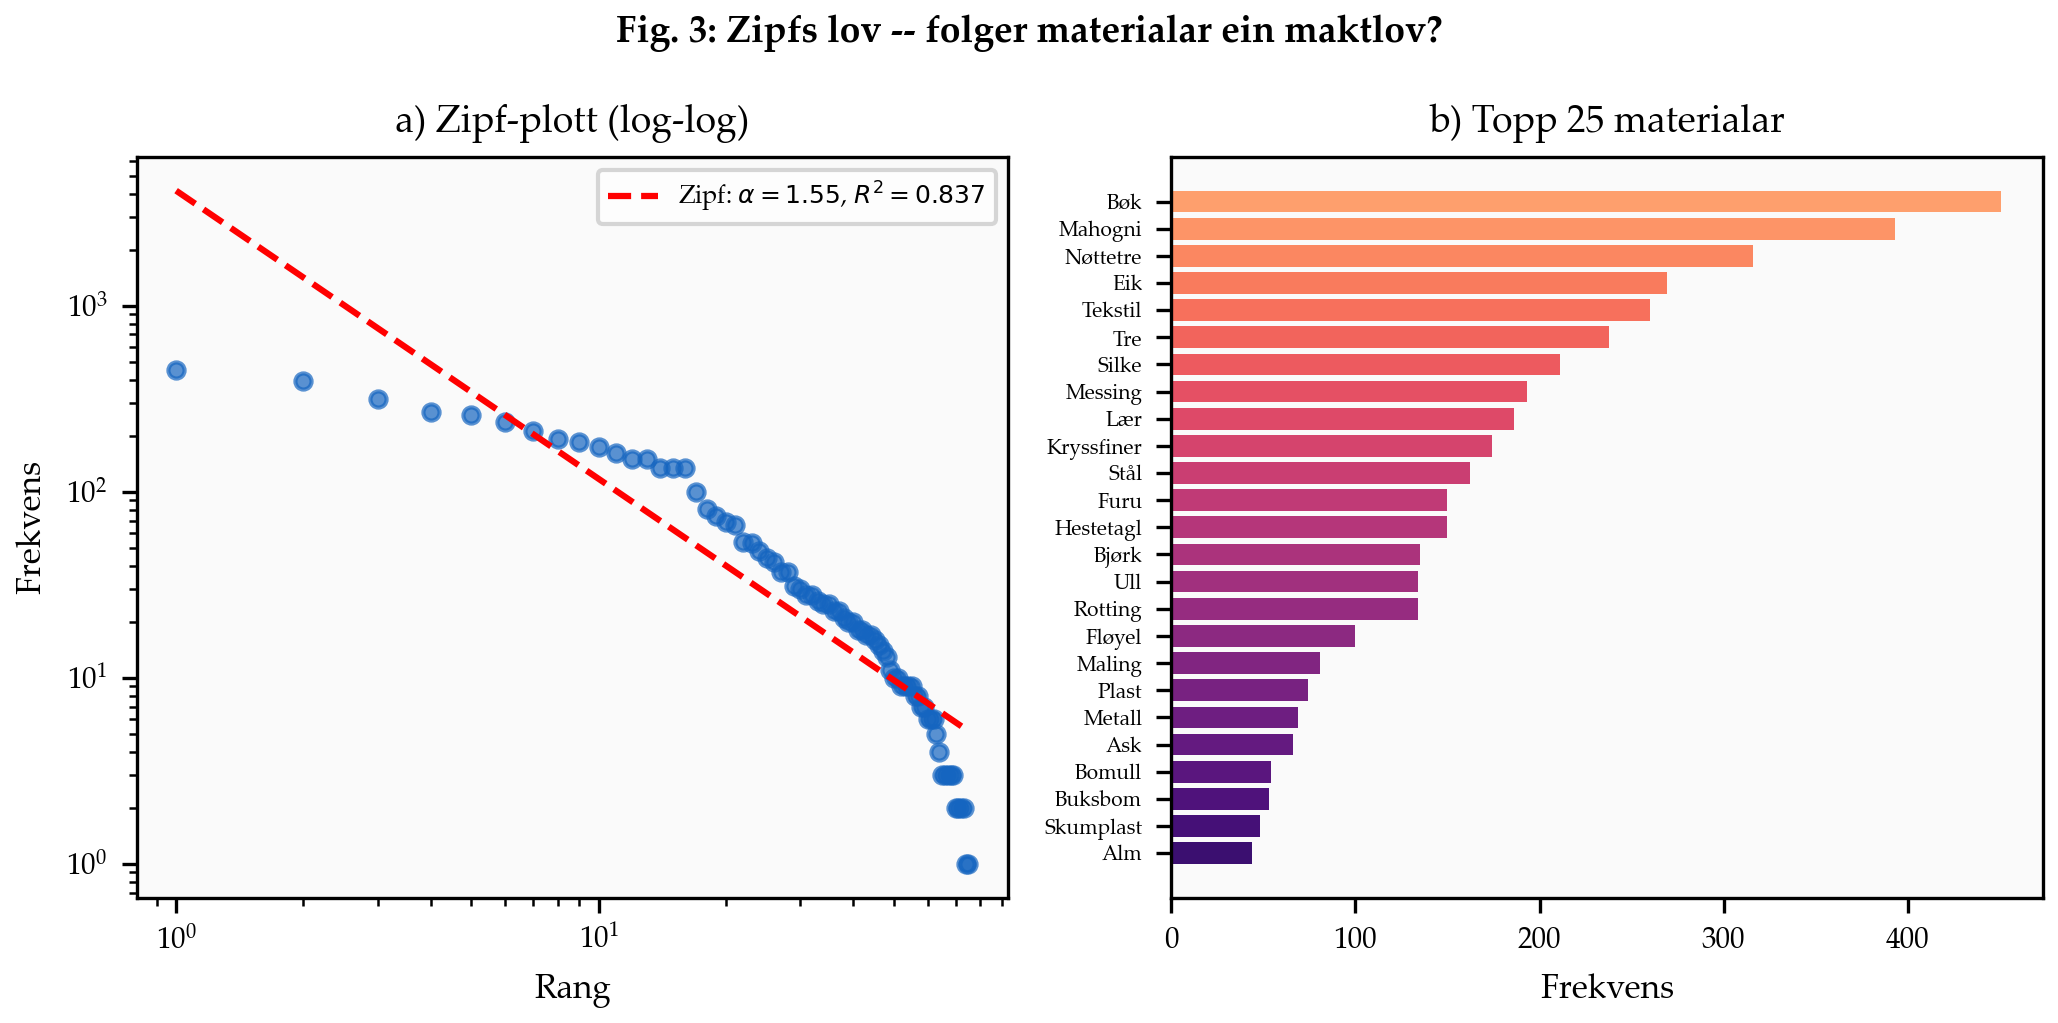
\includegraphics[width=\linewidth]{fig03_zipf.png}
  \caption{Zipf-analyse. (a) Log-log plot: rang vs.\ frekvens. Maktlov-eksponent $\alpha = 1{,}55$, $R^2 = 0{,}84$. (b) Topp~25 materialar.}
  \label{fig:zipf}
\end{figure}

Svaret er \emph{ja}. Materialfordelinga f\o{}lger ein maktlov med eksponent $\alpha = 1{,}55$ ($R^2 = 0{,}84$, $p < 10^{-30}$). Til samanlikning: Zipf-eksponenten for engelsk tekst er typisk $\alpha \approx 1{,}0$, medan $\alpha \approx 1{,}5$ er typisk for \emph{biologiske system} -- artsmangfald i \o{}kosystem \citep{newman2005}.

Implikasjonen er djup: materialfordelinga i stoldesign f\o{}lger ikkje ein ``tilfeldig'' eller ``jamn'' fordeling. Ho f\o{}lger same statistiske lov som artsrikdom i regnskogar og ordfrekvens i romanar. Designkultur er, statistisk sett, eit spr\aa{}k -- og eit \o{}kosystem.

% ── EXP 4 ─────────────────────────────────────────────────────
\subsection{Exp.~4: Materialnettverket}

Me bygger eit nettverks der kvar node er eit materiale og kvar kant representerer kor ofte to materialar opptrer i same stol. Louvain-algoritmen detekterer fellesskap.

\begin{figure}[H]
  \centering
  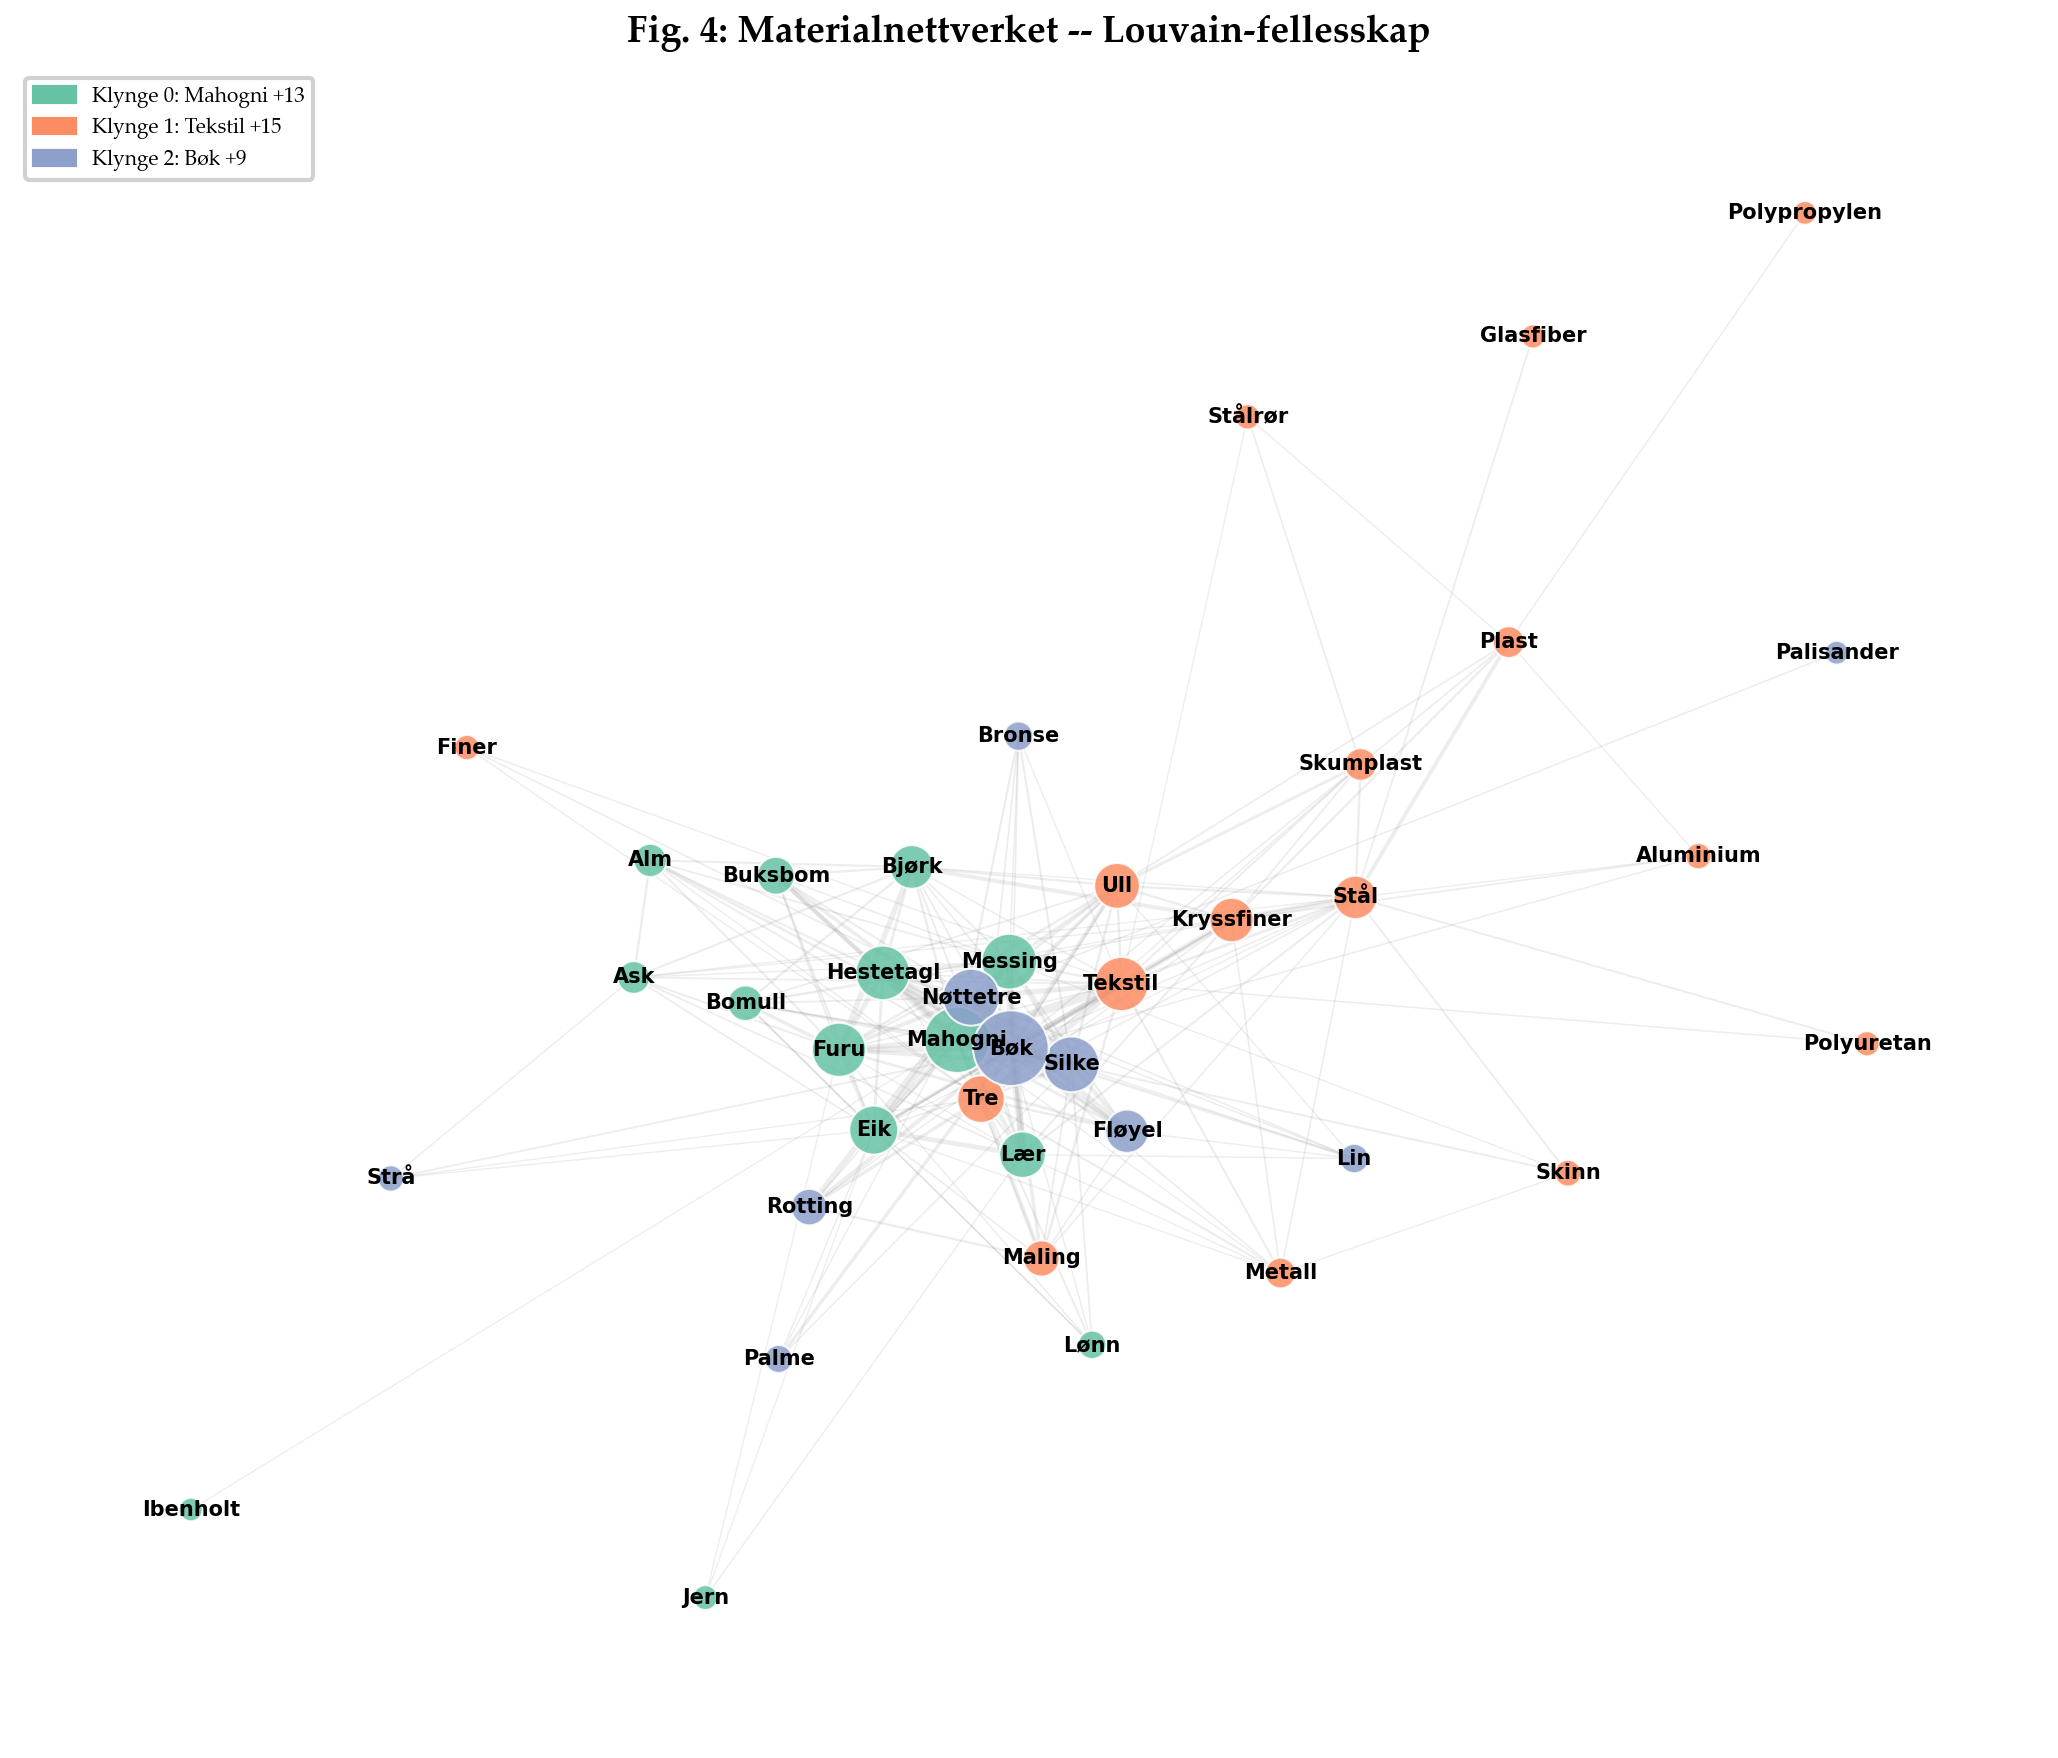
\includegraphics[width=\linewidth]{fig04_nettverk.png}
  \caption{Material-ko-førekomstnettverket (40 nodar, 207 kantar). Tre Louvain-fellesskap: (0) Mahogni--messing--hestetagl (``kolonialt''), (1) Tekstil--st\aa{}l--kryssfiner (``industrielt''), (2) B\o{}k--n\o{}ttetre--silke (``kontinentalt'').}
  \label{fig:network}
\end{figure}

Dei tre fellesskapa korresponderer med distinkte historiske ``materialregime'':

\begin{enumerate}[leftmargin=*, topsep=3pt, itemsep=2pt]
  \item \textbf{Det koloniale fellesskapet} (mahogni, messing, l\ae{}r, hestetagl, furu, eik): materialar knytte til britisk kolonihandel og tradisjonelt snikkarhandverk.
  \item \textbf{Det industrielle fellesskapet} (tekstil, st\aa{}l, maling, kryssfiner, ull): materialar som dominerer etter den industrielle revolusjonen.
  \item \textbf{Det kontinentale fellesskapet} (b\o{}k, n\o{}ttetre, silke, fl\o{}yel, bronse, rotting): materialar typiske for kontinental-europeisk luksushandverk.
\end{enumerate}

At nettverksanalysen \emph{sj\o{}lv} oppdagar desse historiske regima -- utan eksplisitt tidsinformasjon -- er eit sterkt funn. Materialkultur har struktur som er lesbar p\aa{} tvers av tid.

% ── EXP 5 ─────────────────────────────────────────────────────
\subsection{Exp.~5: Granger-kausalitet -- kva driv formendring?}

Granger-kausalitet \citep{granger1969} testar om tidlegare verdiar av variabel $X$ hjelper til med \aa{} predikere framtidige verdiar av variabel $Y$, utover det $Y$ sj\o{}lv kan predikere. Me testar fire variablar: h\o{}gde, breidde, materialtal og materialentropi.

\begin{figure}[H]
  \centering
  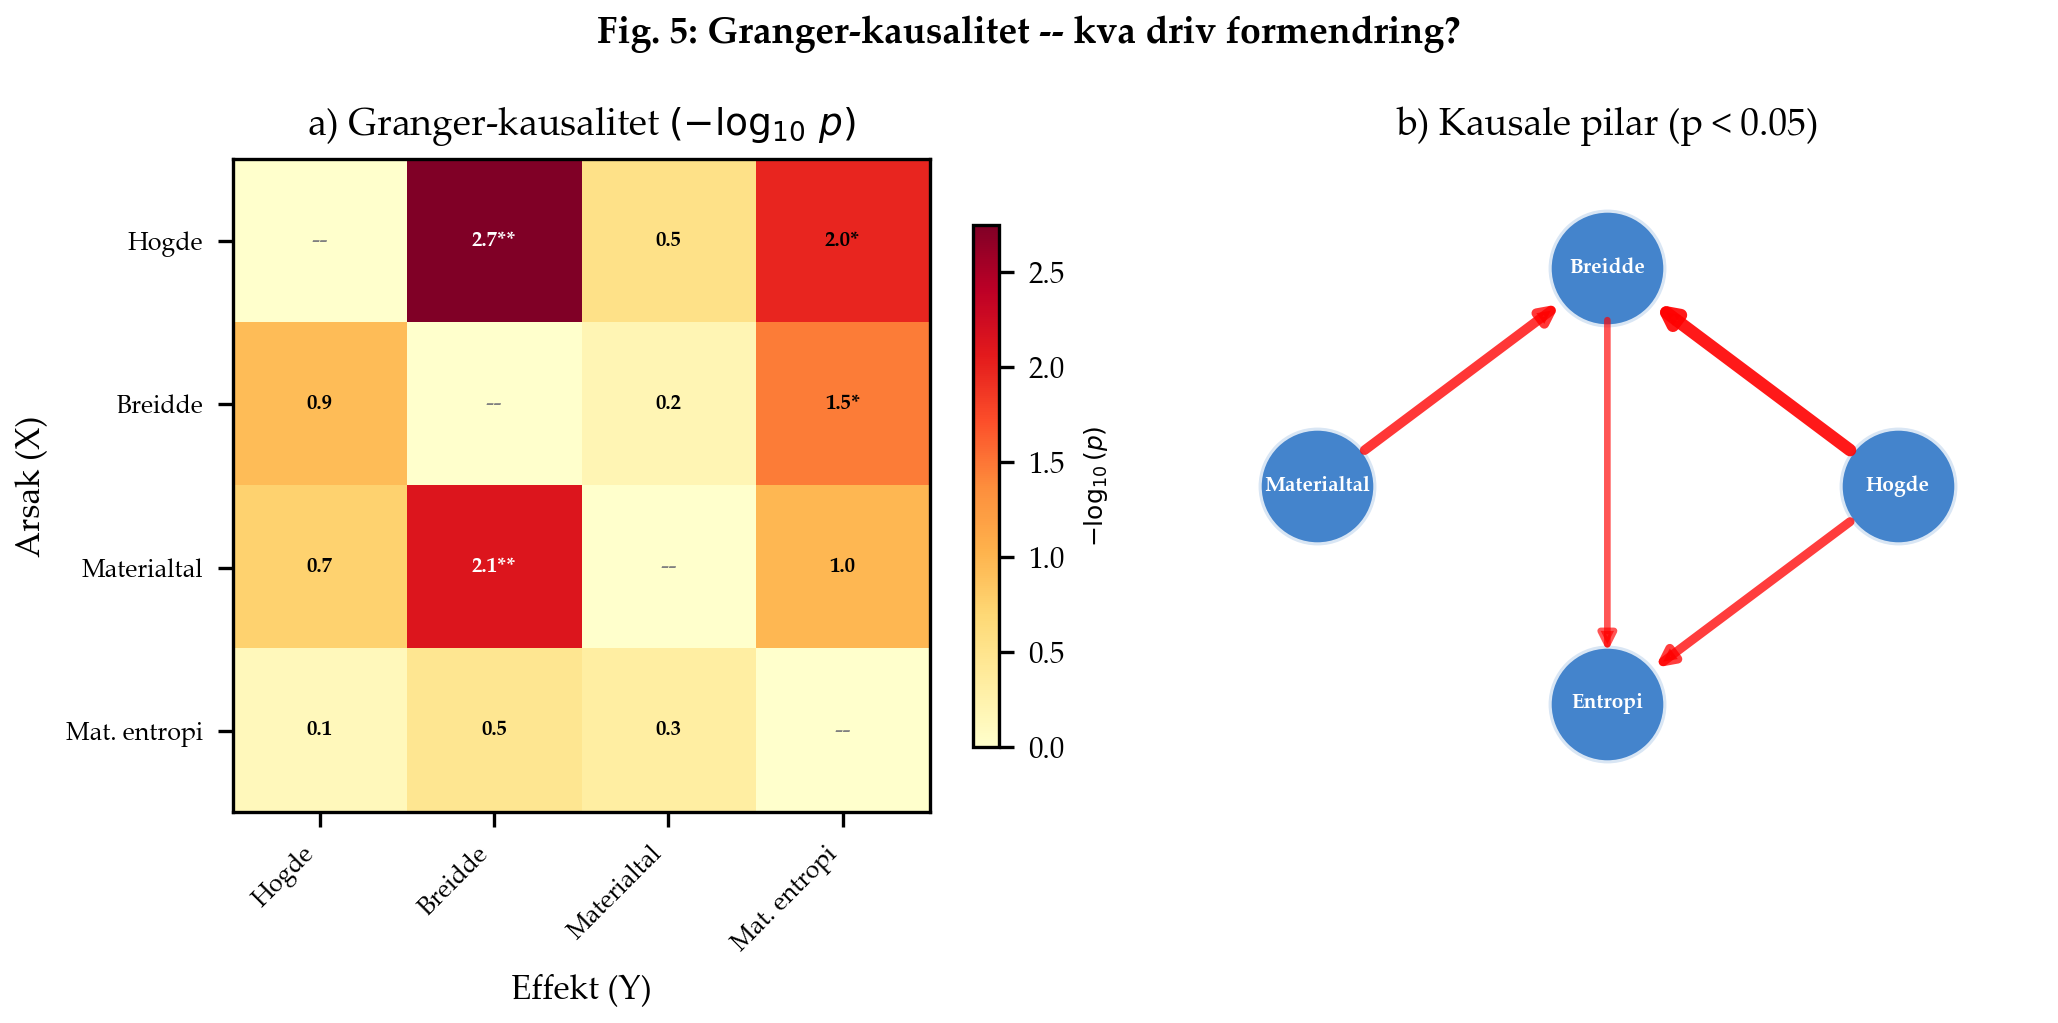
\includegraphics[width=\linewidth]{fig05_granger.png}
  \caption{Granger-kausalitet. (a) Matrise ($-\log_{10} p$, stjerner = signifikans). (b) Kausale pilar. H\o{}gde for\aa{}rsakar breidde og materialentropi; materialtal for\aa{}rsakar breidde.}
  \label{fig:granger}
\end{figure}

Tre kausale lenker er statistisk signifikante:
\begin{itemize}[leftmargin=*, topsep=3pt, itemsep=2pt]
  \item $H \rightarrow W$ ($p = 0{,}002$): H\o{}gdeendring \emph{f\o{}reg\aa{}r} breiddeendring. Stolens vertikale dimensjon leiar.
  \item $H \rightarrow H'_{\mathrm{mat}}$ ($p = 0{,}011$): Dimensjonsendringar driv materialinnovasjon, ikkje omvendt.
  \item $\mathrm{MatCount} \rightarrow W$ ($p = 0{,}008$): Fleire materialar i stolen leiar til breidare stolar -- truleg fordi materialinnovasjon opnar for nye konstruksjonsmetodar.
\end{itemize}

Den kausale retninga er overraskande: \emph{form driv material}, ikkje material driv form. Kausalitetskjeda er: $H \rightarrow W$, $H \rightarrow H'$, $\mathrm{MC} \rightarrow W$. Dimensjonane er ``det som skjer f\o{}rst''.

% ── EXP 6 ─────────────────────────────────────────────────────
\subsection{Exp.~6: Forbodne sonar i morforommet}

\begin{figure}[H]
  \centering
  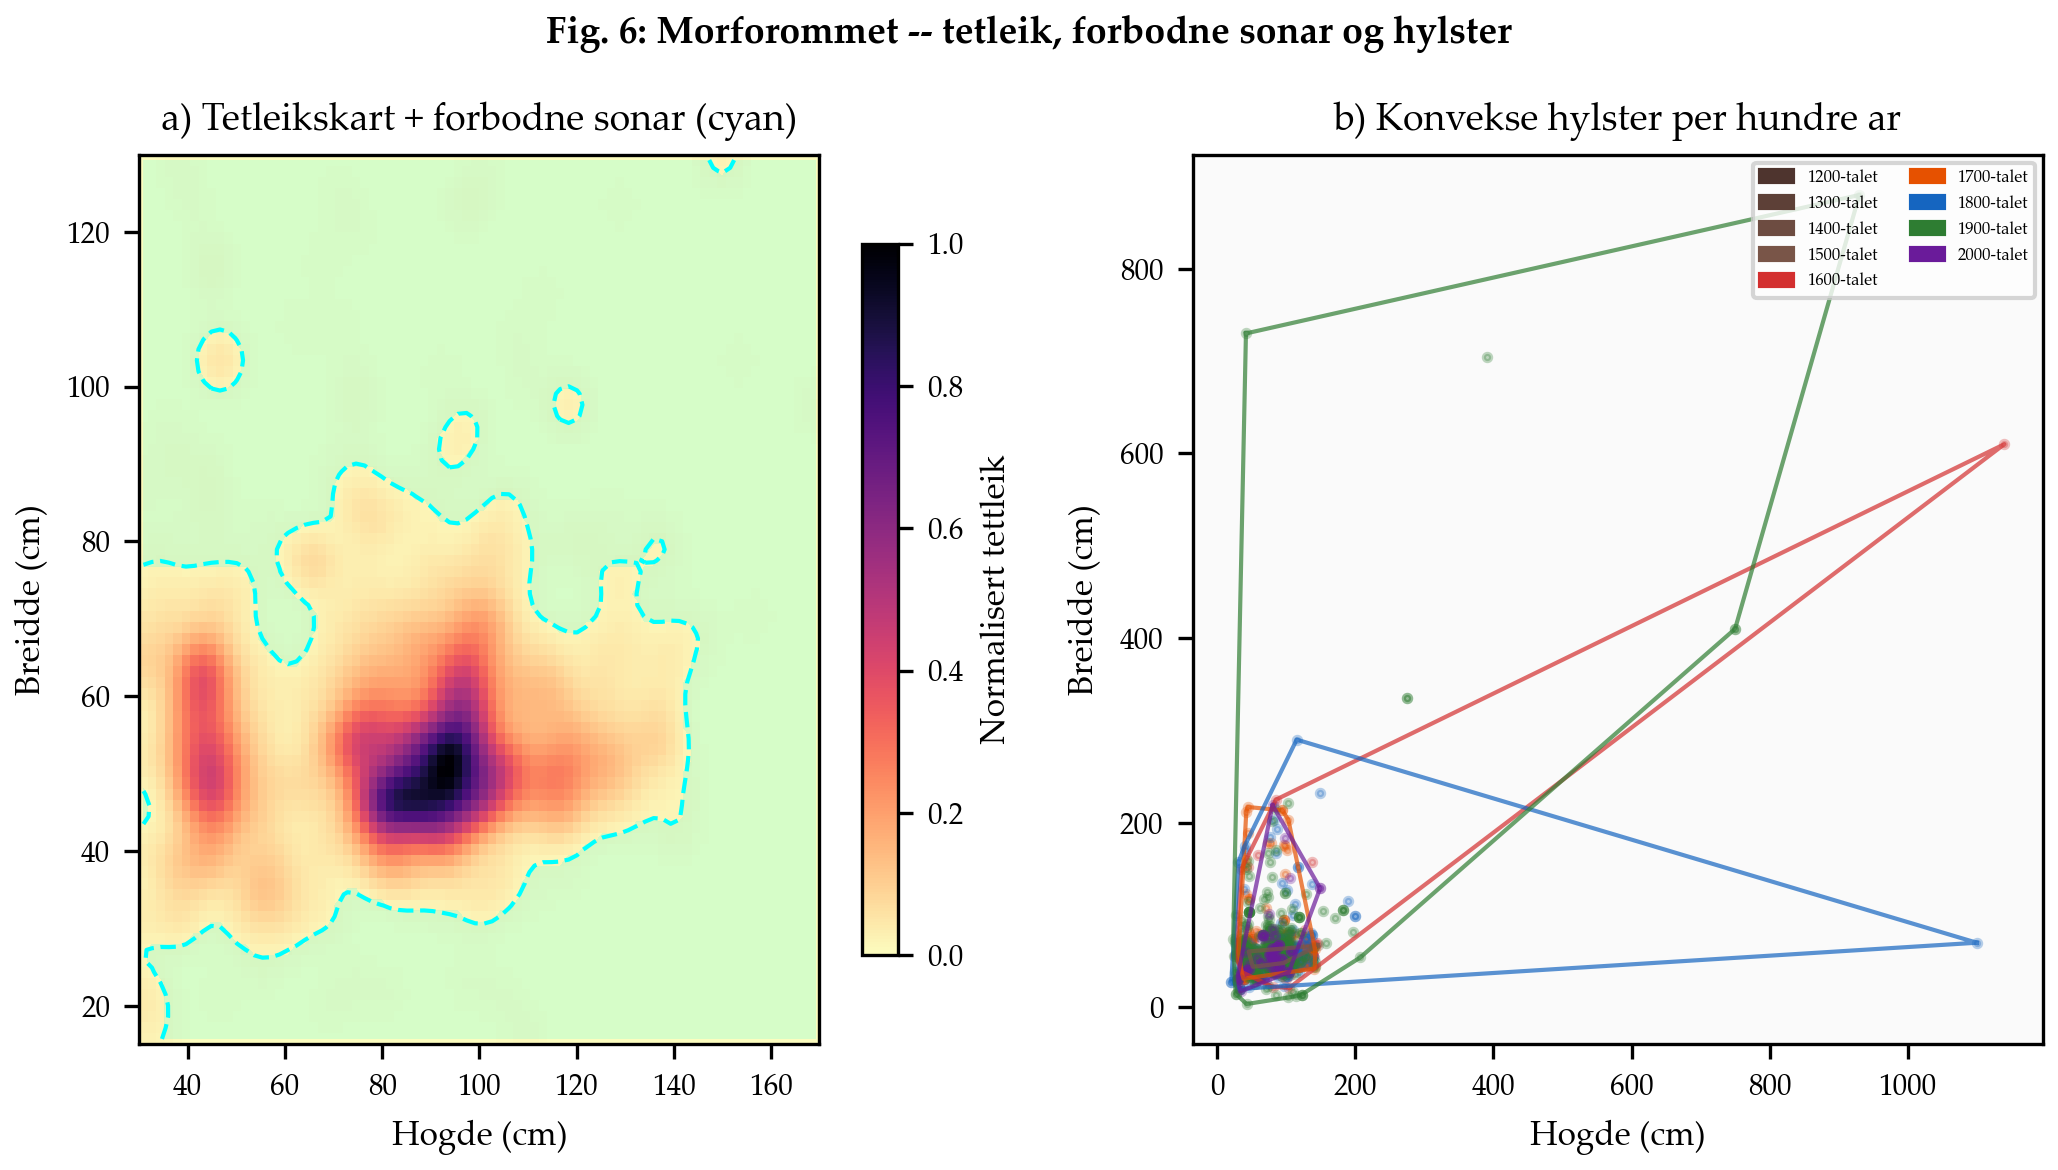
\includegraphics[width=\linewidth]{fig06_voronoi.png}
  \caption{Morforommet. (a) Tetleikskart med forbodne sonar (cyan, $< 2\%$ av maks). \textbf{67{,}7\%} av morforommet er \emph{tomt}. (b) Konvekse hylster per hundre\aa{}r -- 1900-talets hylster er 38$\times$ st\o{}rre enn 1700-talets.}
  \label{fig:voronoi}
\end{figure}

67{,}7\% av det mogelege $(H, W)$-rommet er aldri vorte okkupert av ein einaste stol i 744~\aa{}r. Desse ``forbodne sonane'' representerer kombinasjonar som er ergonomisk, strukturelt eller kulturelt ulevedyktige: ein stol som er 150~cm h\o{}g og 20~cm brei finst ikkje -- og kan truleg ikkje eksistere.

Hundre\aa{}rshylstra avslorer ein dramatisk ekspansjon: 1700-talets konvekse hylster er $15\,587~\mathrm{cm}^2$, medan 1900-talets er $476\,763~\mathrm{cm}^2$ -- ein 31-faldig eksplosjon. Modernismen opna morforommet meir enn nokon annan historisk kraft.

% ── EXP 7 ─────────────────────────────────────────────────────
\subsection{Exp.~7: Mutasjonsrate -- kor raskt muterer stolen?}

Me definerer ``mutasjonsrate'' etter analogi med molekyl\ae{}r evolusjon: dimensjonsmutasjon (absolutt endring i $H + W$ per \aa{}r) og materialmutasjon (Jaccard-avstand mellom tiar).

\begin{figure}[H]
  \centering
  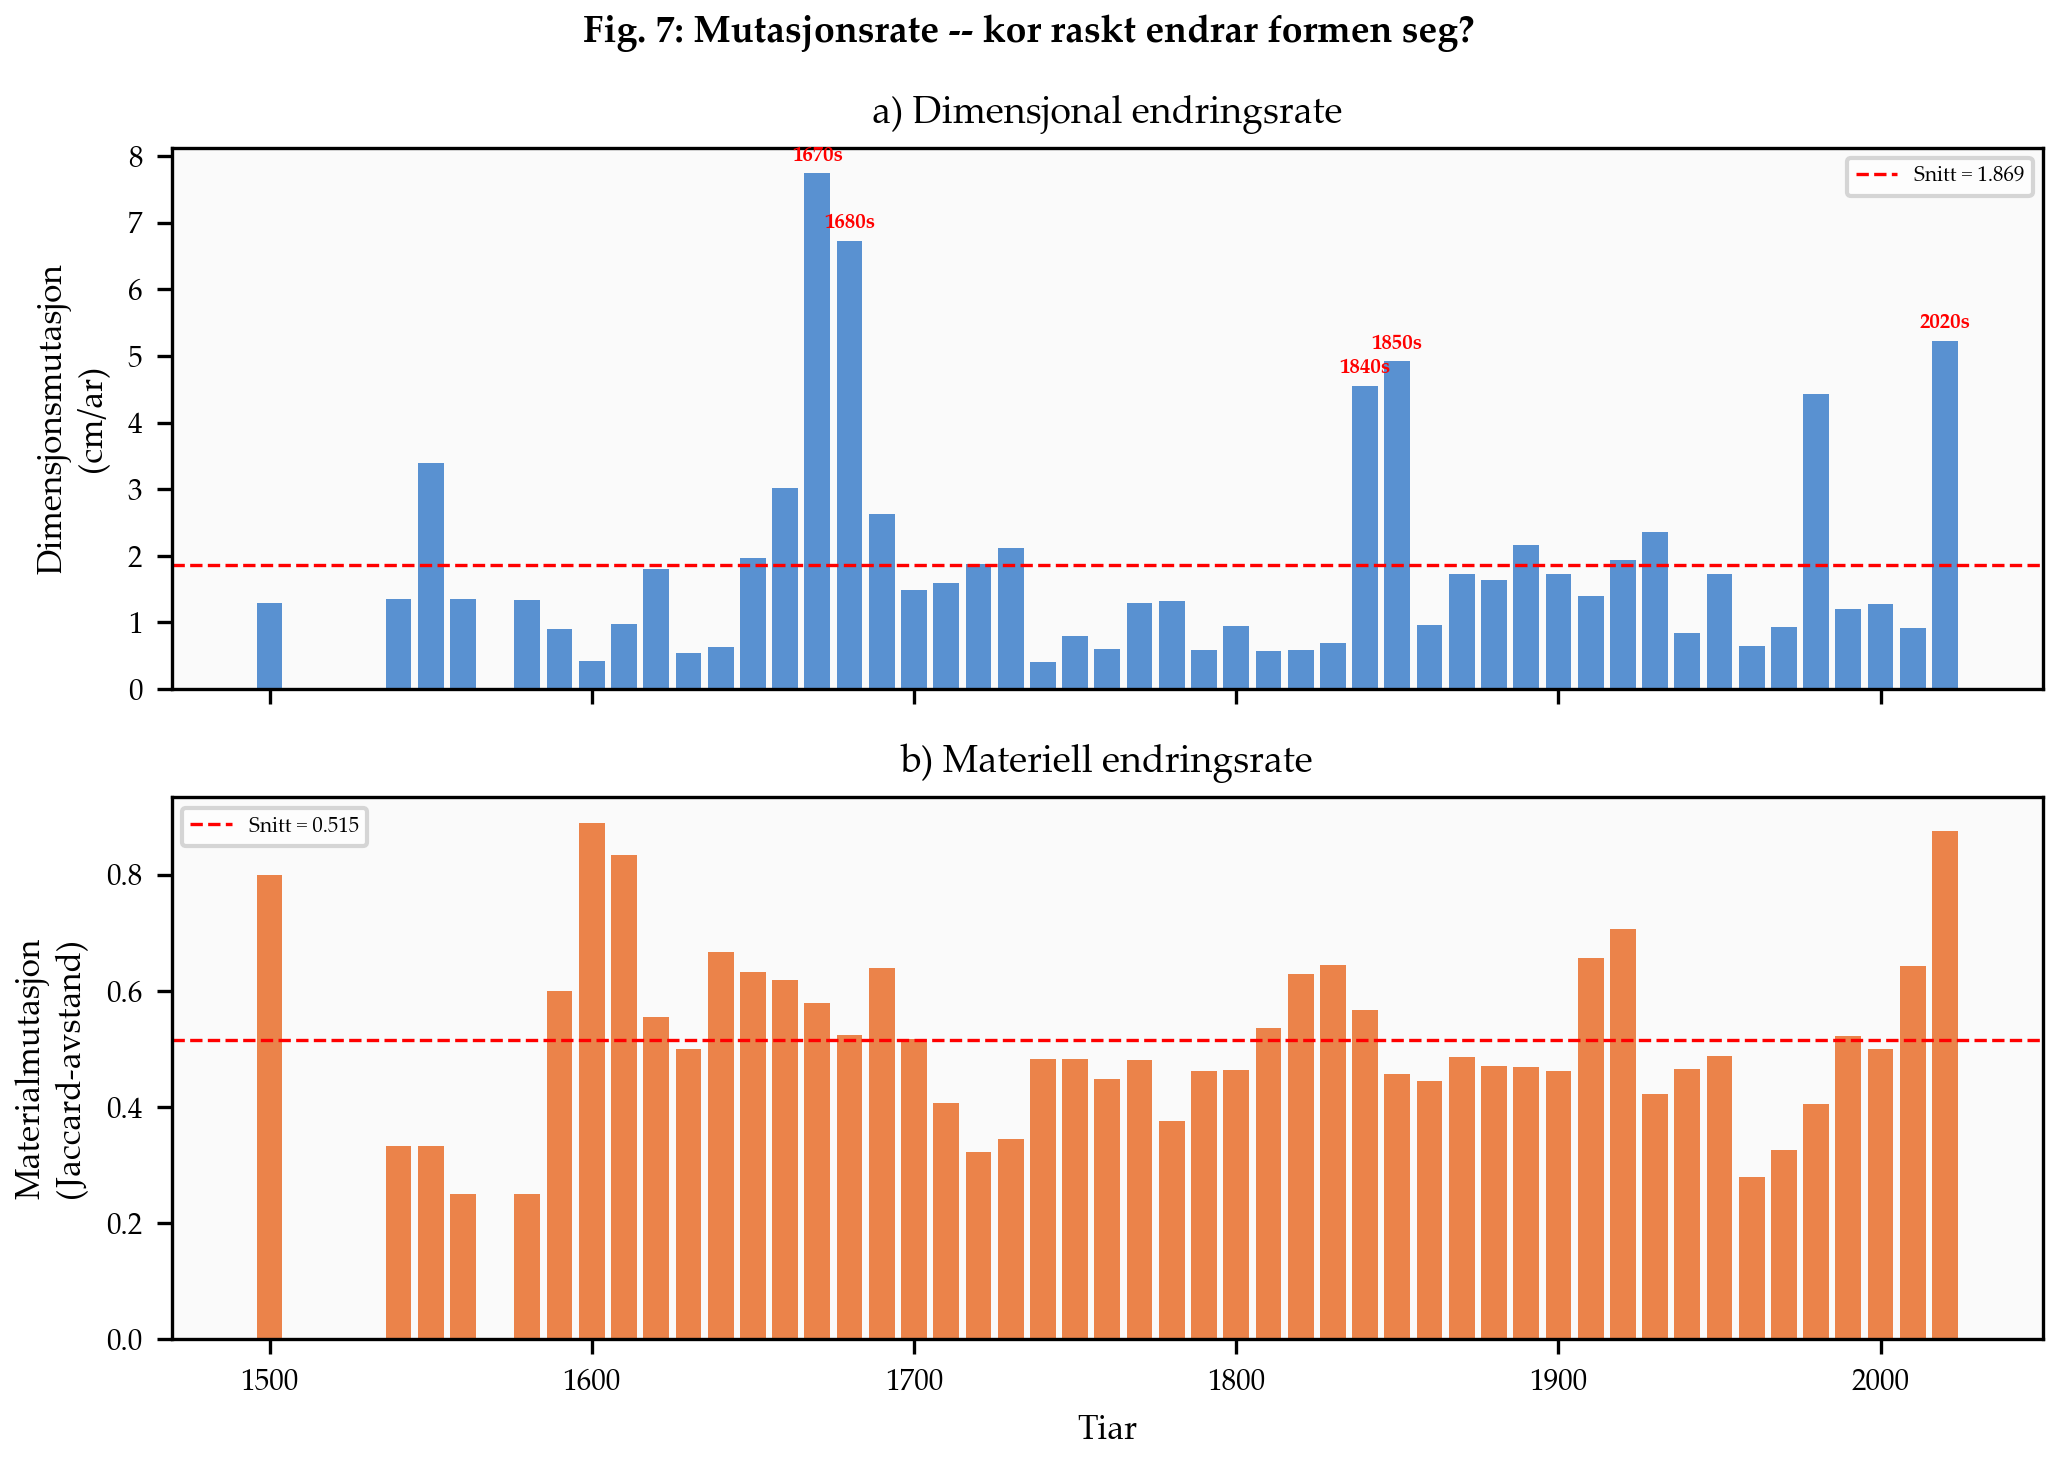
\includegraphics[width=\linewidth]{fig07_mutasjonsrate.png}
  \caption{Mutasjonsrate over tid. (a)~Dimensjonsmutasjon med toppar p\aa{} 1670, 1680, 1840 og 2020. (b)~Materialmutasjon med toppar p\aa{} 1600, 1920 og 2020.}
  \label{fig:mutation}
\end{figure}

Mutasjonsraten er ikkje konstant. Dei st\o{}rste dimensjons\-mutasjonane skjer p\aa{} 1670--1680-talet (barokkens h\o{}gdepunkt), 1840--1850-talet (industrialiseringa) og 2020-talet. Materialmutasjonen toppar p\aa{} 1600 (overgangen fr\aa{} renessanse til barokk), 1920 (modernismens gjennombrot) og 2020 (n\aa{}tid).

Monsteret er klart: \emph{stilskifte er ikkje gradvise prosessar, men punktuerte brot}. Mutasjonsratane er l\aa{}ge i stabile periodar og eksploderer ved overgangane -- pr\aa{}sis slik ``\textbf{punktert likevekt}'' \citep{eldredge1972} beskriv biologisk evolusjon.

% ── EXP 8 ─────────────────────────────────────────────────────
\subsection{Exp.~8: Transfer-entropi -- informasjonsflyt}

Transfer-entropi $TE(X \rightarrow Y)$ m\aa{}ler kor mykje informasjon fr\aa{} tidlegare verdiar av $X$ reduserer uvissa om framtidige verdiar av $Y$, utover det $Y$ sj\o{}lv gir \citep{schreiber2000}.

\begin{figure}[H]
  \centering
  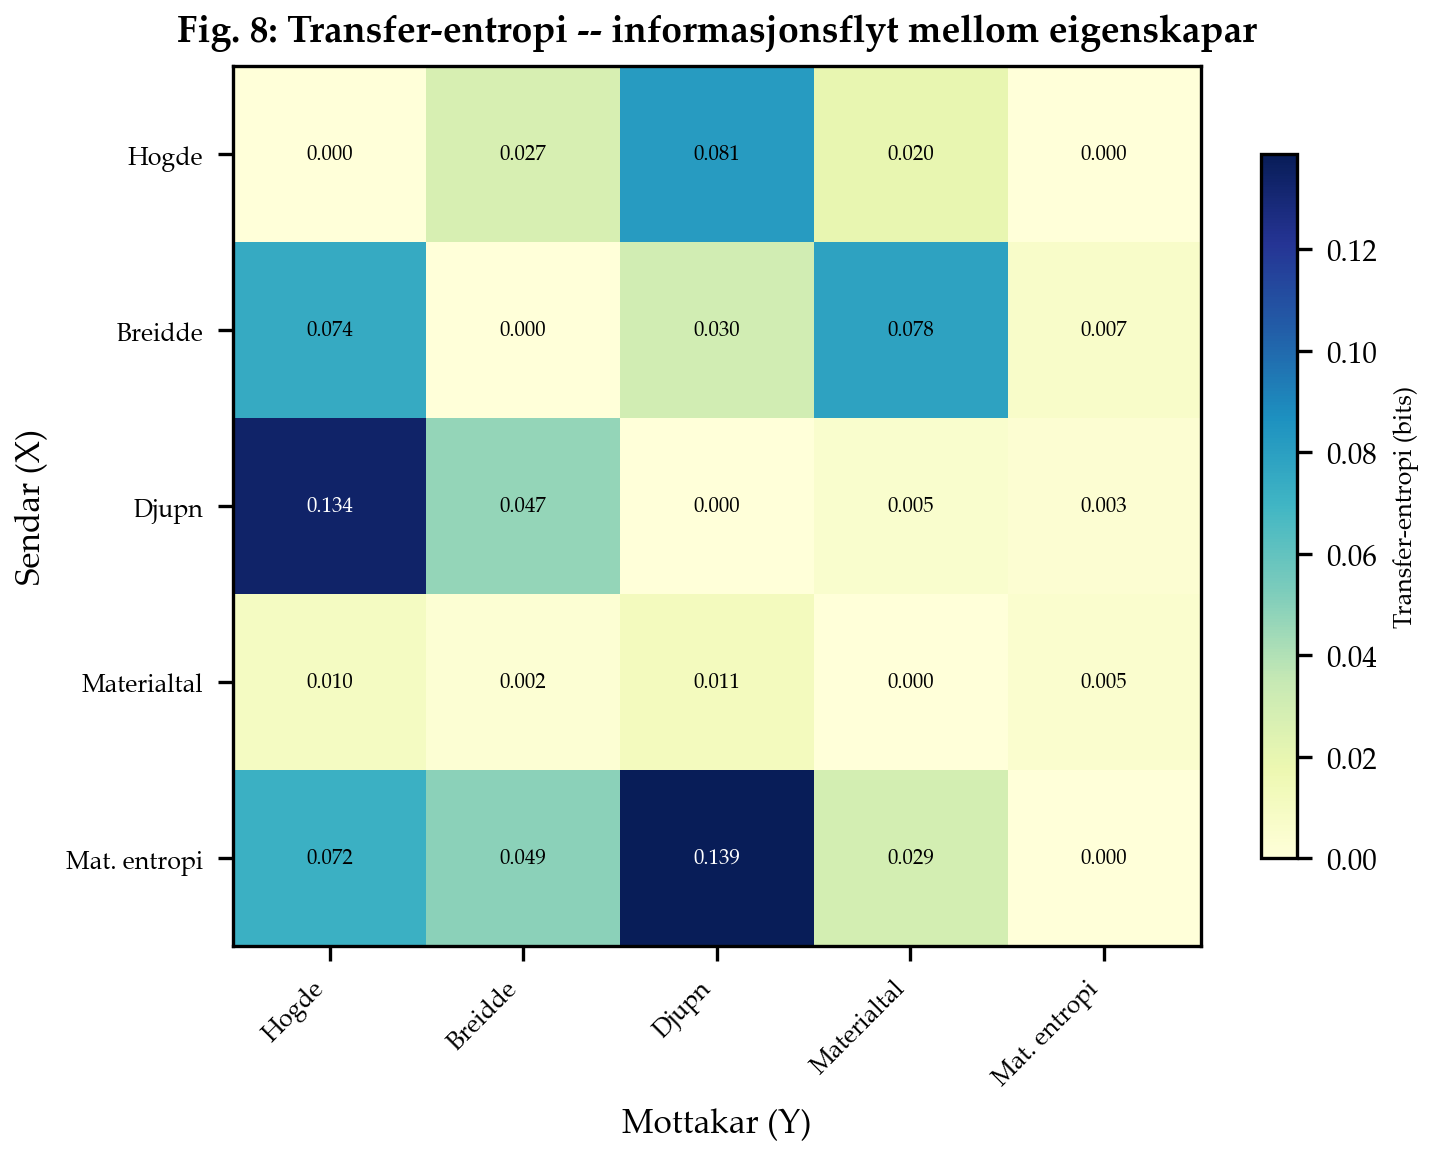
\includegraphics[width=\linewidth]{fig08_transfer_entropi.png}
  \caption{Transfer-entropimatrise. St\o{}rste informasjonsflyt: materialentropi $\rightarrow$ djupn ($TE = 0{,}139$ bits) og djupn $\rightarrow$ h\o{}gde ($TE = 0{,}134$ bits).}
  \label{fig:transfer}
\end{figure}

Den st\o{}rste informasjonsflyten g\aa{}r fr\aa{} materialentropi til djupn ($TE = 0{,}139$ bits) og fr\aa{} djupn til h\o{}gde ($TE = 0{,}134$ bits). Materialentropien er den st\o{}rste \emph{sendaren} av informasjon i systemet: endringar i materialmangfald propagerer ut i alle dimensjonar.

Kausalitetskjeda fr\aa{} Granger-analysen og transfer-entropien gir saman eit samansett bilete: h\o{}gde f\o{}reg\aa{}r breidde (Granger), men materialentropi driv djupn og h\o{}gde (TE). Systemet har \emph{fleire kausale vegar} som opererer p\aa{} ulike tidsskalaer.

% ── EXP 9 ─────────────────────────────────────────────────────
\subsection{Exp.~9: Stilgenomet -- material-DNA}

Me kodar kvar stilperiode som eit bin\ae{}rt ``genom'': eit materiale er ``til stades'' (1) dersom det opptrer i meir enn 10\% av periodans stolar, og ``frav\ae{}rande'' (0) elles.

\begin{figure}[H]
  \centering
  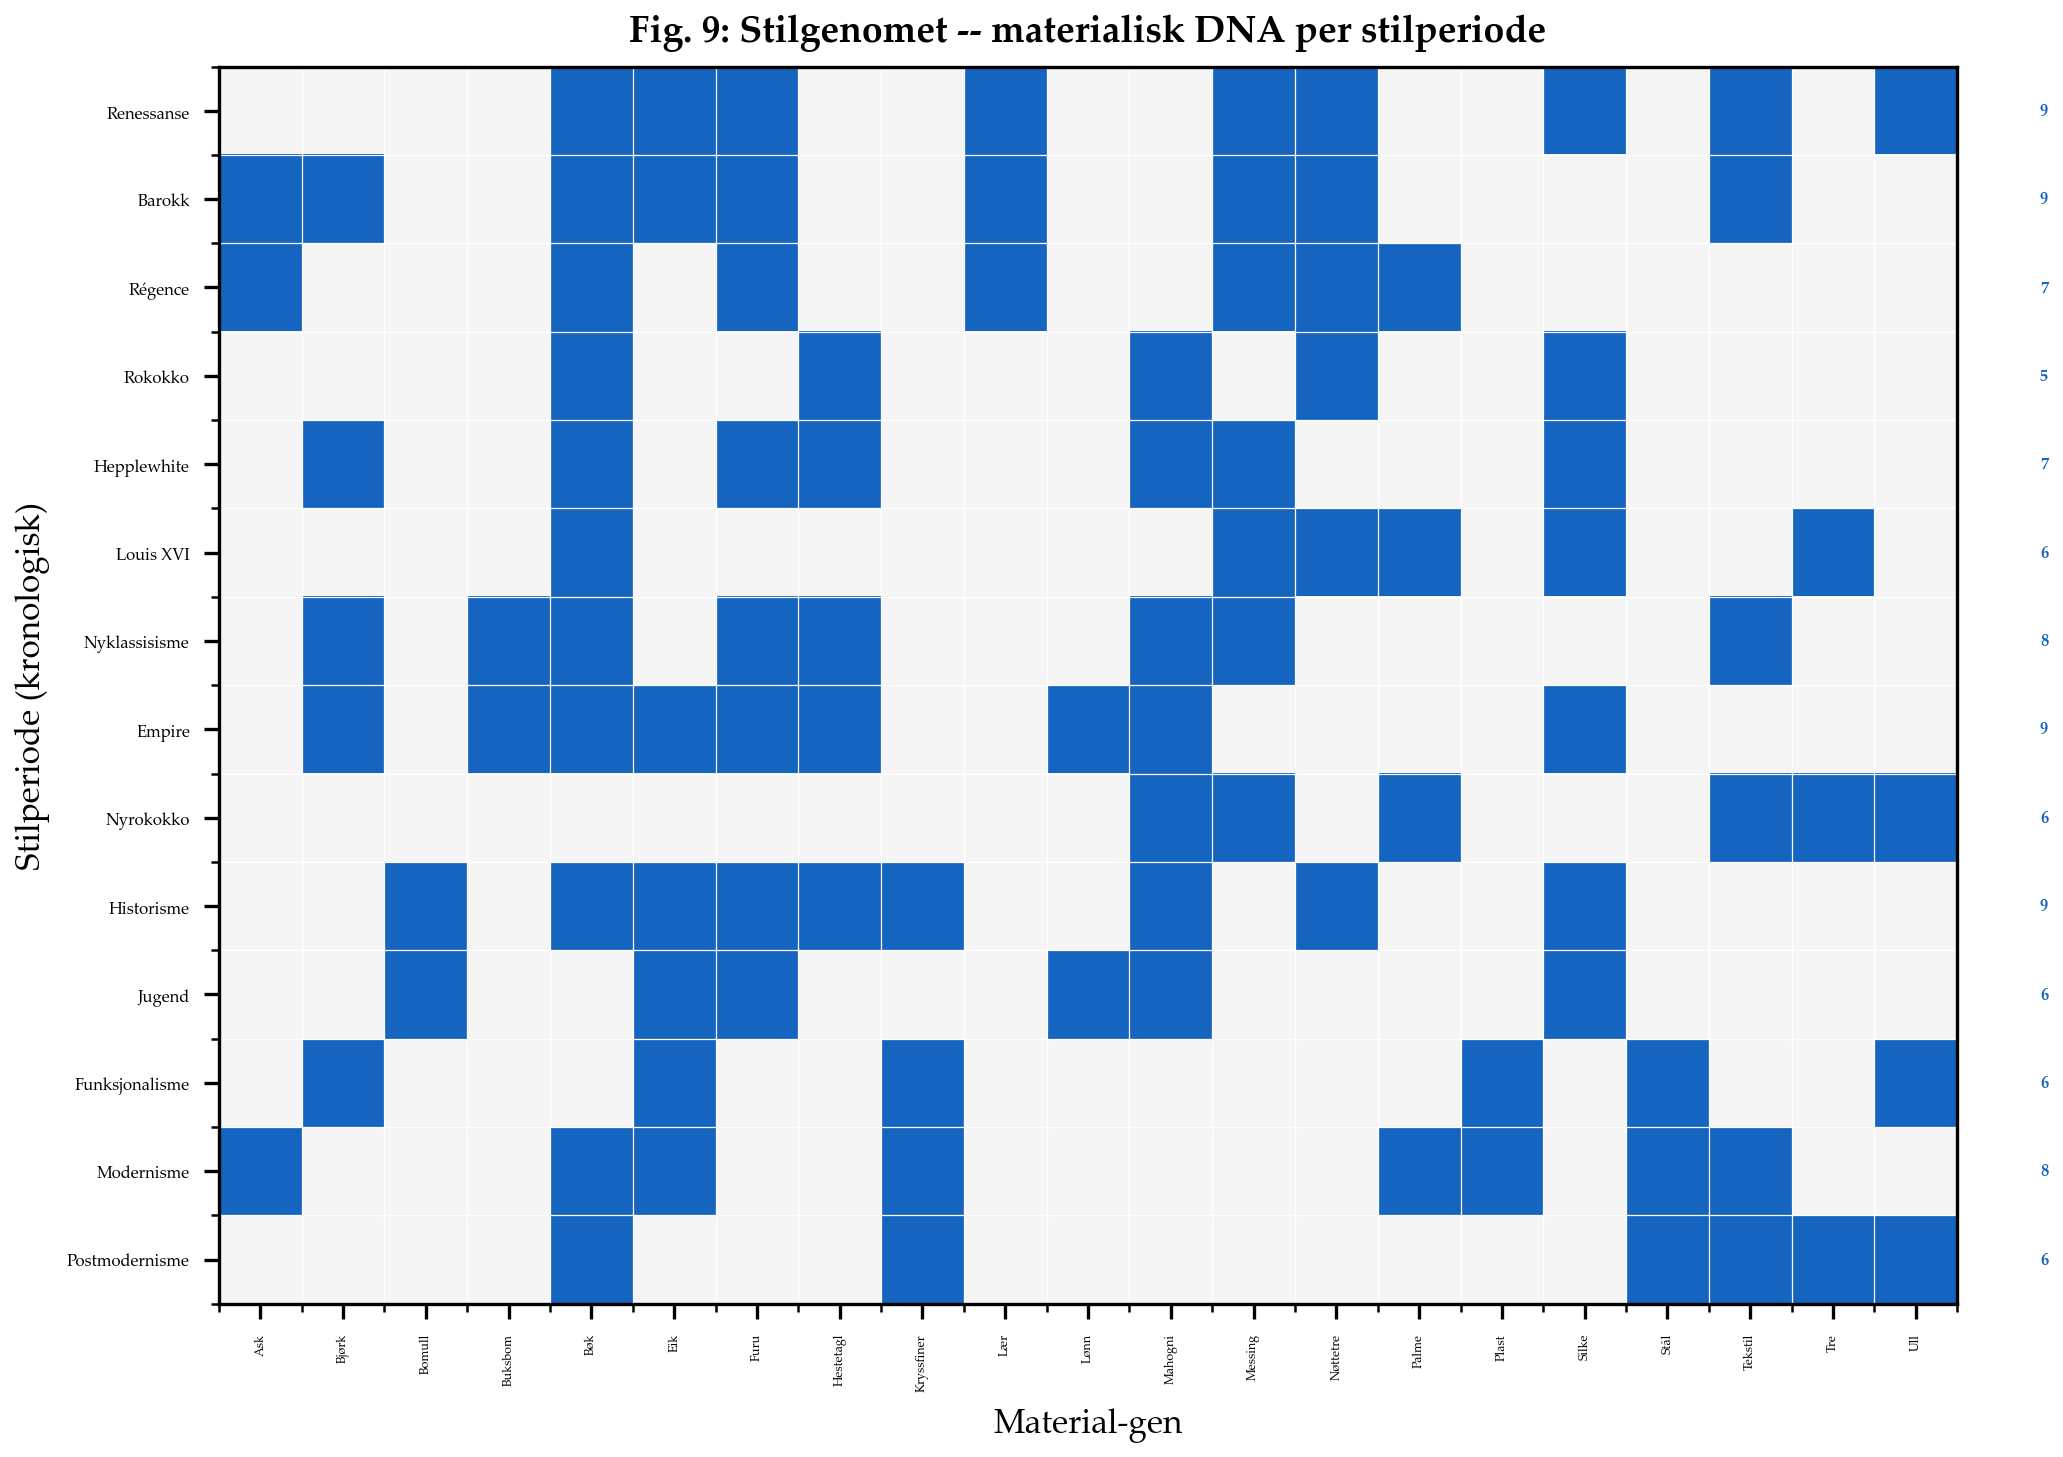
\includegraphics[width=\linewidth]{fig09_genom.png}
  \caption{Stilgenomet: 14 stilperiodar $\times$ 21 aktive material-gen. Bl\aa{} = til stades, kvit = frav\ae{}rande. Ingen einskild gen er universelt konservert; renessansen er mest ``gen-rik'' (9 gen), rokokko mest ``gen-fattig'' (5 gen).}
  \label{fig:genome}
\end{figure}

Det kanskje mest overraskande funnet: \emph{ingen materialar er universelt konserverte}. Det finst ikkje eit einaste materiale som er til stades i alle stilperiodar. Kvar stilperiode har eit unikt ``genom'' -- ein distinkt materiell signatur. Renessansen er den mest ``gen-rike'' stilen (9 aktive material-gen), medan rokokko er mest ``gen-fattig'' (5 gen) -- ein høgt spesialisert periode.

% ── EXP 10 ────────────────────────────────────────────────────
\subsection{Exp.~10: Meisterplottet}

Dei tre mest informasjonsrike aksane -- materialentropi, dimensjonskompleksitet (CV) og Margalef-rikdom -- dannar eit tredimensjonalt rom der 50 tiarsprofilar teiknar ein bane.

\begin{figure}[H]
  \centering
  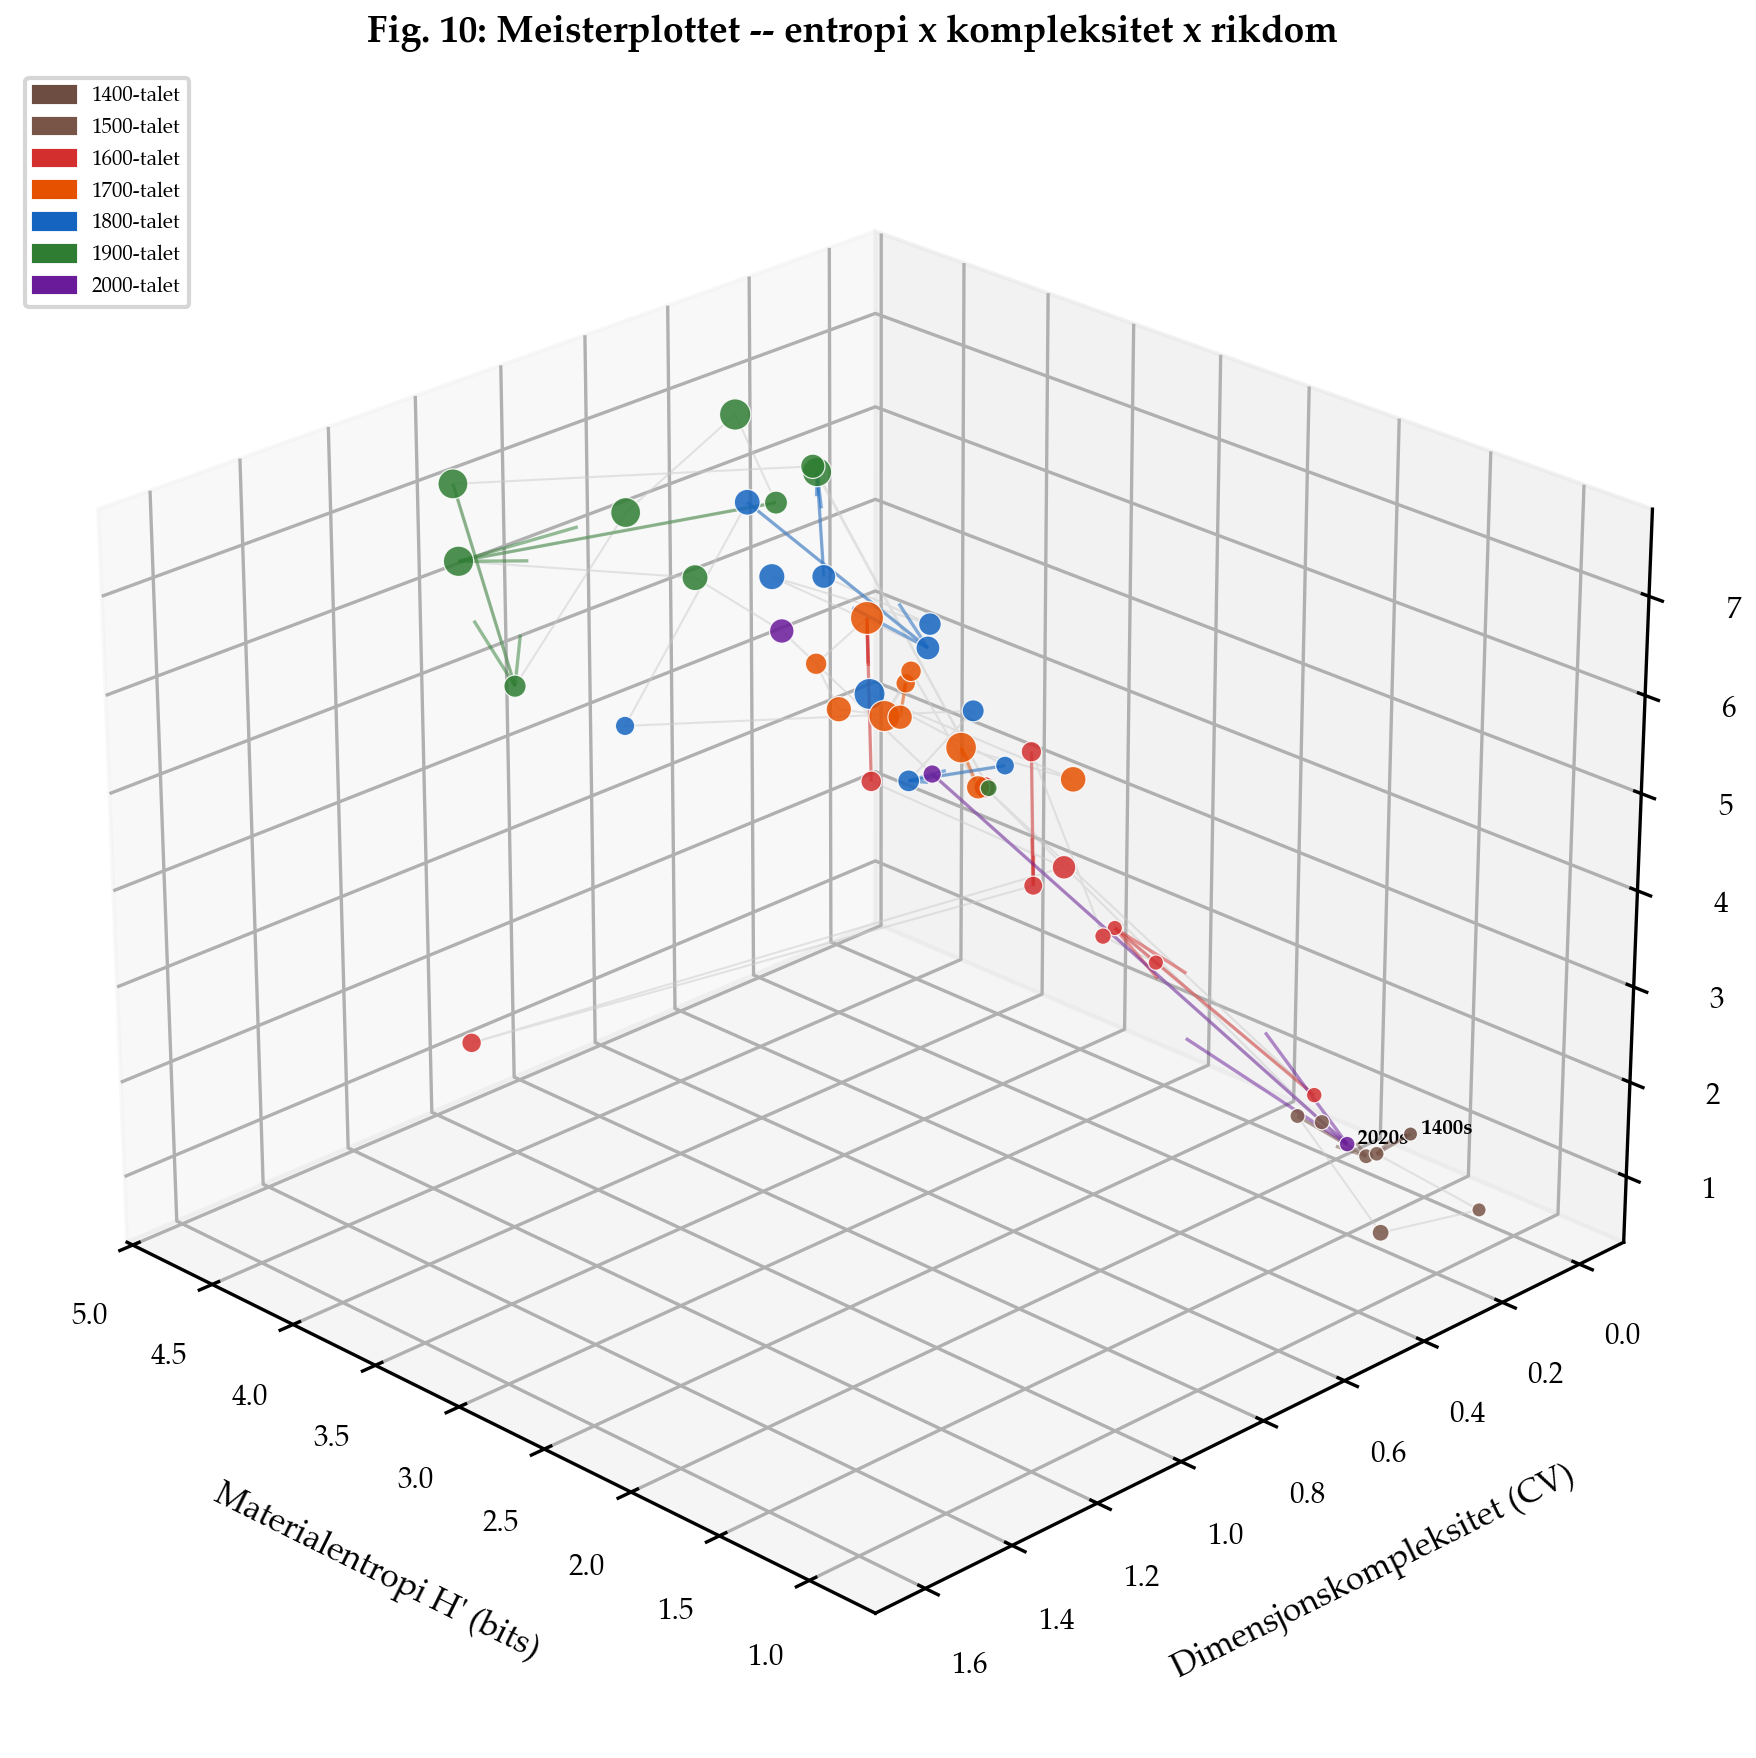
\includegraphics[width=\linewidth]{fig10_meisterplott.png}
  \caption{Meisterplottet: 50 tiar som bane gjennom rommet (entropi $\times$ kompleksitet $\times$ rikdom). Bana g\aa{}r fr\aa{} nedre venstre (l\aa{}g entropi, l\aa{}g kompleksitet) til \o{}vre h\o{}gre (h\o{}g entropi, h\o{}g rikdom) -- men med kraftige svingar.}
  \label{fig:master}
\end{figure}

Bana er ikkje monoton: ho spiralerer og svingar. Entropien veks fr\aa{} 0{,}92 til 4{,}76~bits, men kompleksiteten (CV) g\aa{}r opp \emph{og ned} -- med eit topp p\aa{} 1{,}60 f\o{}r ho fell att. Rikdomen (Margalef) veks fraa 0{,}78 til 7{,}39. Systemet akselererer: seinare tiar dekker meir ``avstand'' per tiarsintervall enn tidlegare.


% ═══════════════════════════════════════════════════════════════
\section{Diskusjon: \aa{} lese stolen som eit komplekst adaptivt system}
% ═══════════════════════════════════════════════════════════════

\subsection{Universelle lover}

Tre av ti eksperiment avslorer universelle statistiske lover: Zipfs maktlov ($\alpha = 1{,}55$), harmoniske syklusar (128/64/32~\aa{}r) og punktuert likevekt i mutasjonsratane. Desse lovene er ikkje spesifikke for stoldesign -- dei opptrer i spr\aa{}k, \o{}kosystem, genom og geologisk stratigrafi. At dei opptrer her tyder p\aa{} at stoldesign ikkje berre er ein kulturprosess: det er eit komplekst adaptivt system \citep{holland1995} som f\o{}lger same organisatoriske prinsipp som andre slike system.

\subsection{Kausal arkitektur}

Granger-kausaliteten og transfer-entropien gir saman ein \textbf{kausal arkitektur}: h\o{}gde leiar breidde (Granger), materialentropi driv djupn (TE), og materialtal driv breidde (Granger). Systemet har fleire kausale skalaer som opererer samstundes. Implikasjonen for designteori er at formendringar ikkje vert drivne av ein einskild faktor (funksjon, estetikk, material) -- dei vert drivne av eit \emph{nettverk av gjensidig p\aa{}verkande krefter}.

\subsection{Dei forbodne sonane}

At 67{,}7\% av morforommet er permanent tomt er kanskje det mest konkrete funnet i denne artikkelen. Det tyder p\aa{} at formrommet har \emph{harde grenser} -- ikkje berre kulturelle preferansar, men fysiske og ergonomiske avgrensingar som definerer kva for formar som er mogelege. Den 31-faldige eksplosjonen av konveks hylster-areal fr\aa{} 1700- til 1900-talet viser at modernismen sine teknologiske innovasjonar (st\aa{}l, plast, laminat) opna opp tidlegare utilgjengelege regionar i morforommet.

\subsection{Genomet: ingen universelle gen}

Fr\aa{} eit genomisk perspektiv er det fascinerande at ingen materialar er universelt konserverte. I biologi er visse gen (t.d.\ rRNA) til stades i \emph{alle} levande organismar. I stoldesign finst ikkje noko tilsvarande ``materialt rRNA''. Kvar epoke oppfinnar sitt eige materielle vokabular fr\aa{} grunnen av. Tre kan verke som ein kandidat for eit ``konservert gen'', men tr\aa{}dstolar, metallstolar og plaststolar bryt denne antaking\-a.


% ═══════════════════════════════════════════════════════════════
\section{Konklusjon}
% ═══════════════════════════════════════════════════════════════

Ti eksperiment, ti svar:

\begin{enumerate}[leftmargin=*, topsep=3pt, itemsep=2pt]
  \item Stilperiodane dannar eit \textbf{fylogenetisk tre} der formlikskap, ikkje kronologi, avgjer slektskap.
  \item Stolen har \textbf{b\o{}lgjelengder}: 128, 64 og 32~\aa{}rs harmoniske syklusar i dimensjonstidsseriane.
  \item Materialar f\o{}lger \textbf{Zipfs lov} ($\alpha = 1{,}55$), same maktlov som naturlege spr\aa{}k og \o{}kosystem.
  \item Materialar organiserer seg i \textbf{tre nettverksfellesskap}: kolonialt, industrielt, kontinentalt.
  \item H\o{}gde \textbf{for\aa{}rsakar} breidde ($p = 0{,}002$); materialtal for\aa{}rsakar breidde ($p = 0{,}008$).
  \item \textbf{67{,}7\%} av morforommet er \emph{forbode sone} -- formm\o{}nster som aldri har eksistert.
  \item Formendring f\o{}lger \textbf{punktuert likevekt}: lange stabile periodar avbrote av eksplosive mutasjonar.
  \item Materialentropi er den st\o{}rste \textbf{informasjonssendaren} i systemet ($TE = 0{,}139$ bits).
  \item Kvar stilperiode har eit unikt materialgenom: \textbf{ingen gen er universelt konserverte}.
  \item Systemets bane i entropi--kompleksitet--rikdom-rommet \textbf{akselererer} over tid.
\end{enumerate}

Samla tyder desse funna p\aa{} at designhistorie er eit komplekst adaptivt system -- ikkje ei forteljing om stilar, men eit dynamisk system med lover, frekvensar, kausalitetskjedar og evolusjon\ae{}re mekanismar. \AA{} ``jailbreake'' ein stol er \aa{} oppdage at det ikkje er ein gjenstand: det er eit \emph{dokument} skrive i eit spr\aa{}k me berre s\aa{} vidt byrjar \aa{} forst\aa{}.


% ═══════════════════════════════════════════════════════════════
\small
\subsection*{Takk}
Forfattaren takkar Nasjonalmuseet og Victoria \& Albert Museum for datatilgang.

\bibliographystyle{plainnat}

\begin{thebibliography}{9}
\bibitem[Eldredge og Gould(1972)]{eldredge1972}
Eldredge, N., \& Gould, S.\,J. (1972). Punctuated equilibria: An alternative to phyletic gradualism. I T.\,J.\,M.~Schopf (Red.), \textit{Models in Paleobiology} (s.~82--115). Freeman.

\bibitem[Finne(2026)]{finne2026}
Finne, I.\,S. (2026). Forml\ae{}re: Ti proposisjonar om formgjeving. \textit{STOLAR Working Papers}, AHO.

\bibitem[Granger(1969)]{granger1969}
Granger, C.\,W.\,J. (1969). Investigating causal relations by econometric models and cross-spectral methods. \textit{Econometrica}, 37(3), 424--438.

\bibitem[Holland(1995)]{holland1995}
Holland, J.\,H. (1995). \textit{Hidden Order: How Adaptation Builds Complexity}. Addison-Wesley.

\bibitem[Newman(2005)]{newman2005}
Newman, M.\,E.\,J. (2005). Power laws, Pareto distributions and Zipf's law. \textit{Contemporary Physics}, 46(5), 323--351.

\bibitem[Schreiber(2000)]{schreiber2000}
Schreiber, T. (2000). Measuring information transfer. \textit{Physical Review Letters}, 85(2), 461--464.
\end{thebibliography}

\end{document}
